\documentclass[12pt,spanish,fleqn,openany,letterpaper,pagesize]{scrbook}

\usepackage[utf8]{inputenc}
%\usepackage[spanish]{babel}%escribir con acentos sin necesidad de comandos \'{} .
\usepackage{fancyhdr}
\usepackage{epsfig}
\usepackage{epic}
\usepackage{eepic}
\usepackage{amsmath}
\usepackage{threeparttable}
\usepackage{amscd}
\usepackage{here}
\usepackage{graphicx}
\usepackage{lscape}
\usepackage{tabularx}
\usepackage{subfigure}
\usepackage{longtable}
\usepackage{amsfonts}
\usepackage{braket} %quantum brackets


\usepackage{rotating} %Para rotar texto, objetos y tablas seite. No se ve en DVI solo en PS. Seite 328 Hundebuch
                        %se usa junto con \rotate, \sidewidestable ....


\renewcommand{\theequation}{\thechapter-\arabic{equation}}
\renewcommand{\thefigure}{\textbf{\thechapter-\arabic{figure}}}
\renewcommand{\thetable}{\textbf{\thechapter-\arabic{table}}}


\pagestyle{fancyplain}%\addtolength{\headwidth}{\marginparwidth}
\textheight22.5cm \topmargin0cm \textwidth16.5cm
\oddsidemargin0.5cm \evensidemargin-0.5cm%
\renewcommand{\chaptermark}[1]{\markboth{\thechapter\; #1}{}}
\renewcommand{\sectionmark}[1]{\markright{\thesection\; #1}}
\lhead[\fancyplain{}{\thepage}]{\fancyplain{}{\rightmark}}
\rhead[\fancyplain{}{\leftmark}]{\fancyplain{}{\thepage}}
\fancyfoot{}
\thispagestyle{fancy}%


\addtolength{\headwidth}{0cm}
\unitlength1mm %Define la unidad LE para Figuras
\mathindent0cm %Define la distancia de las formulas al texto,  fleqn las descentra
\marginparwidth0cm
\parindent0cm %Define la distancia de la primera linea de un parrafo a la margen

%Para tablas,  redefine el backschlash en tablas donde se define la posici\'{o}n del texto en las
%casillas (con \centering \raggedright o \raggedleft)
\newcommand{\PreserveBackslash}[1]{\let\temp=\\#1\let\\=\temp}
\let\PBS=\PreserveBackslash

%Espacio entre lineas
\renewcommand{\baselinestretch}{1.1}

%Neuer Befehl f\"{u}r die Tabelle Eigenschaften der Aktivkohlen
\newcommand{\arr}[1]{\raisebox{1.5ex}[0cm][0cm]{#1}}

%Neue Kommandos
\usepackage{Befehle}
%Inicio del documento. Tener en cuenta que hay archivos auxiliares

\begin{document}
\pagenumbering{roman}
%\newpage
%\setcounter{page}{1}
\begin{center}
\begin{figure}
\centering%

\epsfig{file=HojaTitulo/EscudoUN,scale=1}%
\end{figure}
\thispagestyle{empty} \vspace*{2.0cm} \textbf{\huge
Caminatas cuánticas}\\[6.0cm]
\Large\textbf{Roberto Germán Mesías Larrea}\\[6.0cm]
\small Universidad Nacional de Colombia\\
Facultad de Ciencias, Departamento de Física\\
Bogotá, Colombia\\
2019\\
\end{center}

\newpage{\pagestyle{empty}\cleardoublepage}

\newpage
\begin{center}
\thispagestyle{empty} \vspace*{0cm} \textbf{\huge
Caminatas cuánticas}\\[3.0cm]
\Large\textbf{Roberto Germán Mesías Larrea}\\[3.0cm]
\small Trabajo de grado presentado como requisito parcial para optar al
t\'{\i}tulo de:\\
\textbf{Físico}\\[2.5cm]
Director:\\
Ph.D., Carlos Leonardo Viviescas Ramirez\\[2.0cm]
L\'{\i}nea de Investigaci\'{o}n:\\
Computación Cuántica\\
Grupo de Investigaci\'{o}n:\\
Caos y Complejidad\\[2.5cm]
Universidad Nacional de Colombia\\
Facultad de Ciencias, Departamento de Física\\
Bogotá, Colombia\\
A\~{n}o\\
\end{center}

\newpage{\pagestyle{empty}\cleardoublepage}

\newpage
\thispagestyle{empty} \textbf{}\normalsize
\\\\\\%
\textbf{(Dedicatoria o un lema)}\\[4.0cm]

\begin{flushright}
\begin{minipage}{8cm}
    \noindent
        \small
        Su uso es opcional y cada autor podr\'{a} determinar la distribuci\'{o}n del texto en la p\'{a}gina, se sugiere esta presentaci\'{o}n. En ella el autor dedica su trabajo en forma especial a personas y/o entidades.\\[1.0cm]\\
        Por ejemplo:\\[1.0cm]
        A mis padres\\[1.0cm]\\
        o\\[1.0cm]
        La preocupaci\'{o}n por el hombre y su destino siempre debe ser el
        inter\'{e}s primordial de todo esfuerzo t\'{e}cnico. Nunca olvides esto
        entre tus diagramas y ecuaciones.\\\\
        Albert Einstein\\
\end{minipage}
\end{flushright}

\newpage{\pagestyle{empty}\cleardoublepage}

\newpage
\thispagestyle{empty} \textbf{}\normalsize
\\\\\\%
\textbf{\LARGE Agradecimientos}
\addcontentsline{toc}{chapter}{\numberline{}Agradecimientos}\\\\
Esta secci\'{o}n es opcional, en ella el autor agradece a las personas o instituciones que colaboraron en la realizaci\'{o}n de la tesis  o trabajo de investigaci\'{o}n. Si se incluye esta secci\'{o}n, deben aparecer los nombres completos, los cargos y su aporte al documento.\\

\newpage{\pagestyle{empty}\cleardoublepage}

\newpage
\textbf{\LARGE Resumen}
\addcontentsline{toc}{chapter}{\numberline{}Resumen}\\\\
El resumen es una presentaci\'{o}n abreviada y precisa (la NTC 1486 de 2008 recomienda revisar la norma ISO 214 de 1976). Se debe usar una extensi\'{o}n m\'{a}xima de 12 renglones. Se recomienda que este resumen sea anal\'{\i}tico, es decir, que sea completo, con informaci\'{o}n cuantitativa y cualitativa, generalmente incluyendo los siguientes aspectos: objetivos, dise\~{n}o, lugar y circunstancias, pacientes (u objetivo del estudio), intervenci\'{o}n, mediciones y principales resultados, y conclusiones. Al final del resumen se deben usar palabras claves tomadas del texto (m\'{\i}nimo 3 y m\'{a}ximo 7 palabras), las cuales permiten la recuperaci\'{o}n de la informaci\'{o}n.\\

\textbf{\small Palabras clave: (m\'{a}ximo 10 palabras, preferiblemente seleccionadas de las listas internacionales que permitan el indizado cruzado)}.\\

A continuaci\'{o}n se presentan algunos ejemplos de tesauros que se pueden consultar para asignar las palabras clave, seg\'{u}n el \'{a}rea tem\'{a}tica:\\

\textbf{Ciencia y tecnolog\'{\i}a}: 1) Astronomy Thesaurus Index. 2) Life Sciences Thesaurus, 3) Subject Vocabulary, Chemical Abstracts Service y 4) InterWATER: Tesauro de IRC - Centro Internacional de Agua Potable y Saneamiento.

\textbf{\LARGE Abstract}\\\\
Es el mismo resumen pero traducido al ingl\'{e}s. Se debe usar una extensi\'{o}n m\'{a}xima de 12 renglones. Al final del Abstract se deben traducir las anteriores palabras claves tomadas del texto (m\'{\i}nimo 3 y m\'{a}ximo 7 palabras), llamadas keywords. Es posible incluir el resumen en otro idioma diferente al espa\~{n}ol o al ingl\'{e}s, si se considera como importante dentro del tema tratado en la investigaci\'{o}n, por ejemplo: un trabajo dedicado a problemas ling\"{u}\'{\i}sticos del mandar\'{\i}n seguramente estar\'{\i}a mejor con un resumen en mandar\'{\i}n.\\[2.0cm]
\textbf{\small Keywords: palabras clave en ingl\'{e}s(m\'{a}ximo 10 palabras, preferiblemente seleccionadas de las listas internacionales que permitan el indizado cruzado)}\\

\renewcommand{\tablename}{\textbf{Tabla}}
\renewcommand{\figurename}{\textbf{Gráfica}}
\renewcommand{\listtablename}{Lista de Tablas}
\renewcommand{\listfigurename}{Lista de Gráficas}
\renewcommand{\contentsname}{Contenido}

\tableofcontents{} %Para el índice

%\newcommand{\clearemptydoublepage}{\newpage{\pagestyle{empty}\cleardoublepage}}
\cleardoublepage
\addcontentsline{toc}{chapter}{Lista de figuras} % para que aparezca en el indice de contenidos
\listoffigures % indice de figuras

%\cleardoublepage
%\addcontentsline{toc}{chapter}{Lista de tablas} % para que aparezca en el indice de contenidos
%\listoftables % indice de tablas

%\chapter*{Lista de s\'{\i}mbolos}
\addcontentsline{toc}{chapter}{\numberline{}Lista de s\'{\i}mbolos}
Esta secci\'{o}n es opcional, dado que existen disciplinas que no manejan s\'{\i}mbolos y/o abreviaturas.\\

Se incluyen s\'{\i}mbolos generales (con letras latinas y griegas), sub\'{\i}ndices, super\'{\i}ndices y abreviaturas (incluir s\'{o}lo las clases de s\'{\i}mbolos que se utilicen). Cada una de estas listas debe estar ubicada en orden alfab\'{e}tico de acuerdo con la primera letra del s\'{\i}mbolo.
\section*{S\'{\i}mbolos con letras latinas}
 \label{simbolos}
 \renewcommand{\arraystretch}{1.3}
%\begin{longtable}[l]{*{4}{>{$}l<{$}}p{9cm}}
\begin{longtable}[l]{>{$}l<{$}l>{$}l<{$}>{$}l<{$}}
%\begin{tabular}
\textbf{S\'{\i}mbolo}&\textbf{T\'{e}rmino}&\textbf{Unidad SI}&\textbf{Definici\'{o}n}\\[0.5ex]\hline
\endfirsthead%
\textbf{S\'{\i}mbolo}&\textbf{T\'{e}rmino}&\textbf{Unidad SI}&\textbf{Definici\'{o}n}\\[0.5ex]\hline
\endhead%
      A              &\'{A}rea                                   &\text{m}^{2}                         &\int\int dxdy\\%
      A_{\text{BET}} &\'{A}rea interna del s\'{o}lido                &\frac{\text{m}^{2}}{\text{g}}        &\text{ver DIN ISO 9277}\\%
      A_{\text{g}}   &\'{A}rea transversal de la fase gaseosa    &\text{m}^{2}                         &\text{Ec...}\\%
      A_{\text{s}}   &\'{A}rea transversal de la carga a granel  &\text{m}^{2}                         &\text{Ec...}\\%
      a              &Coeficiente                            &1                                    &\text{Ec...}\\%
      a              &Contenido de ceniza                    &1                                    &\frac{m_{\text{ceniza}}}{m_{\text{bm,0}}}\\%
      c              &Contenido de carbono                   &1                                    &\frac{m_{\text{C}}}{m}\\%
      c              &Longitud de la cuerda                  &\text{m}                             &\text{Figura...}\\
      c              &Concentraci\'{o}n de la cantidad de materia&\frac{\text{mol}}{\text{m}^{3}}      &\frac{n}{V}\\%
      D              &Di\'{a}metro                               &\text{m}                             &\\%
      E_{\text{A}}   &Energ\'{\i}a de activaci\'{o}n                  &\frac{\text{kJ}}{\text{mol}}         &\text{Ec....}\\%
      F              &Fracci\'{o}n de materia vol\'{a}til            &1                                    &\text{ver DIN 51720}\\%
      Fr             &N\'{u}mero de Froude                       &1                                    &\frac{\omega^{2}R}{g_{\text{0}}}\\%
      \overrightarrow{g}&Aceleraci\'{o}n de la gravedad          &\frac{\text{m}}{\text{s}^{2}}        &\frac{d^{2}\overrightarrow{r}}{dt^{2}}\\%
      H              &Entalp\'{\i}a                               &\text{J}                             &U+PV\\%
      H_{\text{o}}   &Poder calor\'{\i}fico superior              &\frac{\text{MJ}}{\text{kg}}          &\text{ver DIN 51857}\\%
      h              &Contenido de hidr\'{o}geno                 &1                                    &\frac{m_{\text{H}}}{m}\\%
      K              &Coeficiente de equilibrio              &1                                    &\text{Ec...}\\%
      L              &Longitud                               &\text{m}                             &DF\\%
      L              &Longitud del reactor                   &\text{m}                             &\text{Figura...}\\%
      m              &Masa                                   &\text{kg}                            &DF\\%
      \dot{m}        &Flujo de masa                          &\frac{\text{kg}}{\text{s}}           &\frac{m}{t}\\%
      n              &Velocidad de rotaci\'{o}n                  &\frac{\text{1}}{\text{s}}            &\frac{\omega}{2\pi}\\%
      n              &Cantidad de materia                    &\text{mol}                           &DF\\%
      P              &Presi\'{o}n                                &\text{Pa}                            &\frac{\vec{F}\cdot\vec{n}}{A}\\%
      Q              &Calor                                  &\text{kJ}                            &\text{1. $LT$}\\%
      T              &Temperatura                            &\text{K}                             &DF\\%
      t              &Tiempo                                 &\text{s}                             &DF\\%
      x_{\text{i}}   &Fracci\'{o}n de la cantidad de materia     &1                                    &\frac{n_{\text{i}}}{n}\\%
      V              &Volumen                                &\text{m}^{3}                         &\int{dr^{3}}\\%
      \vec{u}        &Velocidad                              &\frac{\text{m}}{\text{s}}            &(\frac{dr}{dt},r\frac{d\upsilon}{dt},\frac{dz}{dt})\\%
      w_{\text{i}}   &Fracci\'{o}n en masa del componente i      &1                                    &\frac{m_{\text{i}}}{m_{\text{0}}}\\%
      w_{\text{w,i}} &Contenido de humedad de la sustancia i &1                                    &\frac{m_{\text{\wasser}}}{m_{\text{i,0}}}\\%
      Z              &Factor de gases reales                 &1                                    &\frac{pv}{RT}\\%
\end{longtable}
\vspace{5ex}
\section*{S\'{\i}mbolos con letras griegas}

\begin{longtable}[l]{>{$}l<{$}l>{$}l<{$}>{$}l<{$}}
\textbf{S\'{\i}mbolo}&\textbf{T\'{e}rmino}&\textbf{Unidad SI}&\textbf{Definici\'{o}n}\\[0.5ex] \hline%
\endfirsthead%
\textbf{S\'{\i}mbolo}&\textbf{T\'{e}rmino}&\textbf{Unidad SI}&\textbf{Definici\'{o}n}\\[0.5ex] \hline%
\endhead%
\renewcommand{\arraystretch}{1.3}
 \label{simbolosg}
     \alpha_{\text{BET}}  &Factor de superficie                  &\frac{\text{m}^{2}}{\text{g}}   &(w_{\text{F,waf}})(A_{\text{BET}})\\%
     \beta_{\text{i}}     &Grado de formaci\'{o}n del componente i   &1                               &\frac{m_{\text{i}}}{m_{\text{bm,0}}}\\%
     \gamma               &Wandhaftreibwinkel (Stahlblech)       &1                               &\text{Secci\'{o}n...}\\
     \epsilon             &Porosidad de la part\'{\i}cula             &1                               &1-\frac{\rho_{\text{s}}}{\rho_{\text{w}}}\\%
     \eta                 &mittlere Bettneigungswinkel (St\"{u}rzen) &1                               &\text{Figura...}\\%
     \theta               &\'{A}ngulo de inclinaci\'{o}n de la cama      &1                               &\text{Figura...}\\
     \theta_{\text{O}}    &\'{A}ngulo superior de avalancha          &1                               &\text{Figura...}\\
     \theta_{\text{U}}    &\'{A}ngulo inferior de avalancha          &1                               &\text{Figura...}\\
     \kappa               &Velocidad de calentamientoe           &\frac{\text{K}}{\text{s}}       &\frac{dT}{dt}\\%
     \nu                  &Coeficiente estequiom\'{e}trico           &1                               &\text{ver DIN 13345}\\%
     \rho_{\text{b}}      &Densidad a granel                     &\frac{\text{kg}}{\text{m}^{3}}  &\frac{m_{\text{S}}}{V_{\text{S}}}\;(\text{Secci\'{o}n...})\\
     \rho_{\text{s}}      &Densidad aparente                     &\frac{\text{kg}}{\text{m}^{3}}  &\frac{m_{\text{F}}}{V_{\text{P}}}\;(\text{Secci\'{o}n...})\\
     \rho_{\text{w}}      &Densidad verdadera                    &\frac{\text{kg}}{\text{m}^{3}}  &\frac{m_{\text{F}}}{V_{\text{F}}}\;(\text{Secci\'{o}n...})\\
     \tau                 &Tiempo adimensional                   &1                               &\text{Ec....}\\%
     \Phi_{\text{V}}      &Flujo volum\'{e}trico                     &\frac{\text{m}^{3}}{\text{s}}   &\frac{\Delta V}{\Delta t}\\
     \omega               &Velocidad angular                     &\frac{1}{\text{s}}              &\frac{d\upsilon}{dt}\\

\end{longtable}


\section*{Sub\'{\i}ndices}
\begin{longtable}[l]{>{}l<{}l}
  \textbf{Sub\'{\i}ndice} & \textbf{T\'{e}rmino} \\[0.5ex] \hline%
  \endfirsthead%
  \textbf{Sub\'{\i}ndice} & \textbf{T\'{e}rmino} \\[0.5ex] \hline%
  \endhead%
\renewcommand{\arraystretch}{1.4}\label{simbolosg}

 bm&materia org\'{a}nica\\%
 DR&Dubinin-Radushkevich\\%
 E&Experimental\\%
 g&Fase gaseosa\\%
 k&Condensado\\%
 Ma&Macroporos\\%
 P&Part\'{\i}cula\\%
 p&Poro\\%
 p&Pirolizado\\%
 R&Reacci\'{o}n\\%
 t&Total\\%
 wf&Libre de agua\\%
 waf&Libre de agua y de ceniza\\%
 0&Estado de referencia\\%

\end{longtable}


\setlength{\extrarowheight}{0pt}


\section*{Super\'{\i}ndices}
\begin{longtable}[l]{>{}l<{}l}
  \textbf{Super\'{\i}ndice} & \textbf{T\'{e}rmino} \\[0.5ex] \hline%
  \endfirsthead%
  \textbf{Super\'{\i}ndice} & \textbf{T\'{e}rmino} \\[0.5ex] \hline%
  \endhead%
\renewcommand{\arraystretch}{1.4}\label{simbolosg}

 n &Coeficiente x\\%



\end{longtable}


\setlength{\extrarowheight}{0pt}


\section*{Abreviaturas}
\begin{longtable}[l]{>{}l<{}l}
  \textbf{Abreviatura} & \textbf{T\'{e}rmino} \\[0.5ex] \hline%
  \endfirsthead%
  \textbf{Abreviatura} & \textbf{T\'{e}rmino} \\[0.5ex] \hline%
  \endhead%
\renewcommand{\arraystretch}{1.4}\label{simbolosg}
 1.$LT$&Primera ley de la termodin\'{a}mica\\%
 $DF$    &Dimensi\'{o}n fundamental\\%
 $RFF$   &Racimos de fruta fresca\\%

\end{longtable}


\setlength{\extrarowheight}{0pt}
%\include{Resumen}%\newcommand{\clearemptydoublepage}{\newpage{\pagestyle{empty}\cleardoublepage}}
\pagenumbering{arabic}
\chapter{Introducci\'{o}n}
Simular física cuántica en un computador convencional requiere recursos exponenciales. De allí la idea de construir un computador que manipule la información basado en los principios de la mecánica cuántica. Los computadores cuánticos, además de poder simular física cuántica, también podrán hacer operaciones notables con consecuencias importantes en diversas áreas. 
Es posible que la criptografía sea la aplicación más difundida, a la que se suman la simulación de átomos ultrafríos, el modelamiento de procesos químicos como posible método de desarrollo de nuevos fármacos. Sus características notables son consecuencia del paralelismo y la interferencia.\\

Un objetivo primordial es determinar cuándo los computadores pueden resolver problemas más rápidos que los computadores clásicos. En esta dirección,
los resultados más famosos son el algoritmo de Shor para factorizar números muy grandes cuya complejidad $\mathcal{O}(\log\log N)$, es una ventaja doble exponencial sobre los algoritmos clásicos (ya sean deterministas o probabilísticos), $\widetilde{\Theta}(\sqrt[4]{N})$, y el algoritmo de búsqueda de Grover que presenta una mejora cuadrática $\mathcal{O}(\sqrt{N})$ sobre el caso clásico $\mathcal{O}(N)$. De esta misma forma, las caminatas cuánticas pueden concretar mejoras exponenciales para diversos probelmas.\\

Las caminatas aleatorias modelan la traslación de un caminante sobre una distribución de vértices en la cual la dirección de cada paso se escoge como resultado de un evento aleatorio. 
Muchos modelos en la ciencia se basan en las caminatas aleatorias. En física la ecuación de Langevin o el movimiento browniano contienen distintos modelos de las caminatas aleatorias, en biología las descripciones de los movimientos de un individuo animal, en ciencias de la computación son una poderosa herramienta que sirve de base para la construcción de algoritmos.\\

Las caminatas cuánticas son procesos análogos a las caminatas aleatorias clásicas, lo que hace natural que presenten un alto poder práctico. El caso cuántico resulta interesante por varias razones: (1) sirven como modelo para procesos en diferentes áreas: por ejemplo la fotosíntesis, la difusión cuántica y el bombeo óptico [Kitakawa, 2005]; (2) mejoran el desempeño de los algoritmos clásicos; (3) son un modelo universal para computación cuántica [Childs, 2009, Lovett, 2010], equivalente, por ejemplo, al modelo de compuertas cuánticas de las máquinas de Turing; y (4) para su implementación no es necesario un computador cuántico.\\

Las caminatas clásicas y cuánticas presentan diferencias en varios aspectos y a varios niveles de sus análisis. Resalta, por su extrañeza, que la distribución de probabilidad del caso cuántico es bimodal a comparación de la distribución gaussiana. Además, y más importante, la varianza de la caminata cuántica es del orden del número de pasos $\mathcal{O}(t)$, mientras que el caso clásico es del orden de la raíz cuadrada del número de pasos $\mathcal{O}(\sqrt{t})$. Tras este resultado, es de esperar que la difusión sobre cualquier espacio que contenga la caminata sea mayor cuando es cuántica. Si a esto le sumamos cualidades como la superposición y la coherencia, las diferencias son definitivas: los algoritmos cuánticos presentan soluciones sin equivalente clásico a ciertos problemas, y mejoras en eficiencia inclusive exponenciales.\\

Sobre grafos las diferencias se evalúan en otros conceptos: algunos son el \textit{mixing time} que es el tiempo que tarda una caminata en converger hacia una distribución límite, y el \textit{hitting time} que es el tiempo en hallar un subconjunto marcado. En la búsqueda sobre el hipercubo (relacionado con el \textit{hitting time}), \cite{shenvi2003quantum} mostró que las caminatas cuánticas son capaces de mejorar cuadráticamente el desempeño de \textit{cualquier} algoritmo clásico. Por su parte, \cite{childs2003exponential} encontró un algoritmo que propaga al caminante, sobre un tipo de grafo de árboles ligados, exponencialmente más rápido que \textit{cualquier} algoritmo clásico. En estos ejemplos la complejidad es mejor no sólo a comparación de las contrapartes clásicas basadas en caminatas aleatorias, pero de cualquier tipo de algoritmo.\\

Con base en caminatas sobre grafos adecuados, las caminatas cuánticas son capaces de resolver problemas de la computación como: búsqueda espacial, problema de colisión sobre grafos, problema de distinción de elementos, \textit{NAND tree evaluation}, \textit{single-source shortest path},   \textit{triangle finding problem}, etc. \cite{shao}. Ambainis et. al \cite{ambainis2007quantum} obtuvieron un algoritmo óptimo para resolver el problema de la distinción de elementos que usa caminatas cuánticas. Szegedy \cite{szegedy2004quantum} propuso un marco general para las caminatas sobre grafos valioso para la búsqueda espacial. Estos dos algoritmos fueron un modelo para la construcción de otros. En cualquier cadena de Markov simétrica y ergódica, el marco de Szegedy logra una mejora cuadrática sobre cualquier algoritmo clásico. Otra marco de búsqueda común es el desarrollado por Magníez et. al \cite{magniez2011search}, llamado MNRS, con el que se descubrieron algoritmos veloces como el de \textit{triangle finding problema} que busca reconocer una estructura triangular en alguna parte del grafo, \textit{group commutative test}, etc.\\

En el trabajo exploramos las caminatas sobre la línea y sobre grafos finitos e infinitos, y resaltamos sus similitudes y diferencias, con énfasis en aquello que destaca a la caminata cuántica en la construcción de los algoritmos.
Está dividido en cuatro partes. En la primera presentamos los modelos las características fundamentales de las caminatas clásicas y las cadenas de Markov. En la parte dos estudiamos la caminata cuántica sobre la línea y definimos los elementos básicos para el análisis y caracterizamos el operador de evolución temporal.
Posteriormente, en la parte tres, las caminatas sobre redes finitas y su dinámica, y presentamos la solución particular para ciertas gráficas. En la cuarta parte, presentamos algunos algoritmos con atención especial en algunos marcos técnicos para los problemas de búsqueda espacial.\\

La revisión de algunos conceptos básicos de la mecánica cuántica: el carácter determinista de la evolución unitaria, la aleatoriedad asociada a la medida, la superposición natural en los espacios de Hilbert, el entrelazamiento entre grados de libertad de un mismo sistema, y los niveles de decoherencia como puente entre lo clásico y lo cuántico, que puede ser un soporte técnico para la optimización de las caminatas. La implementación de las caminatas en algoritmos cuánticos presenta ideas básicas de computación cuántica. En el apéndice se presentan el algoritmo de Grover, óptimo para búsqueda en un conjunto desordenado, algo del álgebra para computación cuántica y circuitos cuánticos.\\


\section{Caminatas aleatorias clásicas}\label{CaminatasClasicas}
El espacio de movimientos puede ser espacio euclídeo. La longitud de los pasos es siempre la misma, y un paso se da cada cierto intervalo de tiempo igual. Es posible hacer las cantidades tan pequeñas como se quiera y considerar tiempo y espacio continuos.\\
Estudiaremos la posición de una partícula tras seguir una caminata de esta naturaleza: con pasos de igual longitud sobre la línea infinita, y una moneda como evento aleatorio. Nos interesa conocer la posición de la partícula.\\

%Emergencia de la simetría rotacional.Ecuación de difusión. Polímeros y caminatas aleatorias. Invarianza de escala, y universalidad. 

\subsection{Caminata aleatoria clásica sobre una recta.}

Si las probabilidades de ir a derecha o izquierda son iguales a $1/2$, y la posición de inicio es $x_0=0$, 
\begin{equation}
\langle x\rangle=0,\quad \langle x_ix_j\rangle=l^2\delta_{i,j}
\end{equation}{}
Después de $t$ pasos, la varianza $\sigma^2=tl^2$:
\begin{equation}{}
\sigma^2=\Big \langle \big(\sum_i^t x_i \big)^2 \Big \rangle = \sum_{i,j}^t \langle x_i x_j \rangle = tl^2,
\end{equation}
El valor esperado de la posición crece como $\sqrt{N}$, $\sigma\sim \sqrt{N}$. Si pensamos en $t$ como el tiempo,\\
Veamos cómo emerge el límite continuo:
\begin{equation}
    \langle\Delta y^i\rangle=\int d^D \Delta y [\Delta y p(\Delta \Vec{y})]=0,
\end{equation}{}

\begin{equation}
    \langle\Delta y^i\Delta y^j\rangle=\int d^D \Delta y [\Delta y^i\Delta y^jp(\Delta \Vec{y})]=\langle(\Delta y)^2\rangle\frac{\delta_{i,j}}{D}
\end{equation}{}

\begin{equation}
P_N(\Vec{x})=\int d^D \Delta y P_{N-1}(\Vec{x}-\Delta \Vec{y})p(\Delta \Vec{y})    
\end{equation}{}

\begin{equation}
    \frac{\partial\rho}{\partial t}=K\nabla^2\rho
    \end{equation}{}
que es la ecuación de difusión, cuya solución es gausiana: $\rho(x,t)=\frac{e^{-x^2/4Kt}}{(4\pi Kt)^{D/2}}$. Esta ecuación macroscópica es un comportamiento emergente de las caminatas aleatorias, lo que significa que es un comportamiento muy independiente de  Otra característica emergente de estas caminatas es que en tiempos muy grandes su escala es invariante, que corresponde a un \textit{fractal}.

\subsection{Caminata sobre una red}
\begin{equation}
    P_N(\Vec{x})=\int_{-\pi}^\pi\frac{d^Dk}{(2\pi)^D}[\cos{(\Vec{k}\cdot\Vec{x})}]\prod_{n=1}^{N}p_n(\Vec{k})
\end{equation}{}
\begin{equation}
    P_N(\Vec{x})=\int_{-\pi}^\pi\frac{d^Dk}{(2\pi)^D}[\cos(\Vec{k}\cdot\Vec{x})]\left(\frac{1}{D}\sum_{j=1}^D\cos{k_j}\right)^N
\end{equation}{}
\begin{equation}
    P_N(J)=\frac{1}{2^N}\frac{N!}{(1/2(N+J))!(1/2(N-J))!}
\end{equation}{}

\begin{equation}
    P_N=\int_{-\pi}^\pi\frac{dk_1}{(2\pi)[\cos{(k_1J)}](\cos{k_1})^N}
\end{equation}{}
\subsection{Dependencia de la dimensión}
Presentemos un curioso resultado relacionado con la dimensión del espacio. 

\begin{equation}
    \mathcal{R}=\sum_{n=0}^\infty u_n
\end{equation}{}

\begin{equation}
    \mathcal{R}=\sum_{k=1}^\infty ku^{k-1}(1-u)=(1-u)^{-1}
\end{equation}{}

\begin{equation}
    u_n=\int_{-\pi}^\pi \frac{d^Dk}{(2\pi)D}\left(\frac{1}{D}\sum_{j=1}^D\right)^n
\end{equation}{}
\begin{equation}
    \mathcal{R}=\sum_{n=0}^\infty u_n=\int_{-\pi}^\pi\frac{d^Dk}{(2 \pi)^D}\left(1-\frac{1}{D}\sum_{j=0}^D\cos k_j\right)^{-1}
\end{equation}{}
\begin{equation}
    \mathcal{R}\approx 2D\int_{k\approx0}\frac{dk_1\dots dk_D}{(2\pi)^D}(k_1^2+\cdots+k_D^2)^{-1}\frac{2D}{(2\pi)^D}\int_{k\approx0}\frac{k^{D-1}dk}{k^2}
\end{equation}{}
Para $D=3$, la integral Watson:
\begin{align}
    \mathcal{R}&=\frac{2}{(2\pi)^3}\int_{-\pi}^\pi dk_1\int_{-\pi}^\pi dk_2\int_{-\pi}^\pi dk_3[3-(\cos k_1+\cos k_2 +\cos k_3)]^{-1}\\
    &=\frac{\sqrt{6}}{32\pi^3}\Gamma(\frac{1}{24})\Gamma(\frac{5}{24})\Gamma(\frac{7}{24})\Gamma(\frac{11}{24})
\end{align}{}
Para 1 dimensión:
\begin{equation}
    u_{2n}=^{2n}C_n\frac{1}{2^{2n}},
\end{equation}{}
usando la aproximación de Stirling para factoriales $n!\approx \sqrt{2\pi n}e^{-n}n^n$ para obtener $u_{2n}\approx 1/\sqrt{\pi n}$,
\begin{equation}
    m=\sum_nu_{2n}=\sum_n\frac{1}{\sqrt{\pi n}}=\infty
\end{equation}{}
Para D=2 el resultado es el cuadrado de D=1,

\begin{equation}
u_n(\Vec{x})=\frac{1}{(2\pi)^D}\frac{1}{2^n}\int_{-\pi}^\pi dk_1\int_{-\pi}^\pi dk_2(\cos{k_1}+\cos{k_2})^n   
\end{equation}
con un cambio de variables $(k_1,k_2)\xrightarrow{}(k_1+k_2,k_1-k_2)$, la integral es el producto de dos integrales para el caso D=1.

\subsection{Cadenas de Markov}
Un proceso estocástico en un espacio de estados discreto $X$, de tamaño $n=|X|$, es una cadena de Markov. Se describe por una \textit{matriz estocástica} $P$, en la que $p_{ab}\in [0,1]$ es la probabilidad de transición de $a$ a $b$, y para todo $a$:
\begin{equation}
    \sum_{b\in X}p_{ab}=1
\end{equation}
Toda cadena de Markov tiene un \textit{grafo dirigido subyacente} con $n$ vértices etiquetados con los nombres de $X$ y arcos dirigidos etiquetados con las probabilidades no nulas $p_{xy}$. La distribución de probabilidad sobre los vértices se representa por un vector fila $\Vec{u}$ con elementos reales no negativos que suman $1$. $\vec{u}$ se transforma con una aplicación de $P$ según $\vec{u}P=\Vec{v}$. Cuando $\vec{\pi}P=\vec{\pi}$, llamamos \textit{distribución estacionaria} a $\vec{\pi}$.\\

\noindent Una cadena de Markov es:
\begin{itemize}
    \item \textit{irreducible}, cuando cualquier vértice del grafo subyacente puede ser alcanzarse en un número de pasos finito
    \item \textit{aperiódica}
    \item \textit{ergódica} si es irreducible y aperiódica.
\end{itemize}
Falta \textit{reversible}\\
\textbf{Teorema de Perron-Froebenious}: Sea $P$ una matriz estocástica. Entonces:
\begin{itemize}
    \item todos los autovalores de $P$ son a lo más $1$ en valor absoluto y $1$ es un autovalor de $P$;
    \item si $P$ es irreducible, entonces el 1-autovector es único y estrictamente positivo (esto es, es de la forma $c\vec{\pi}$, donde $c\neq 0$ y $\vec{\pi}$ es una distribución no nula en todas las entradas);
    \item si además de ser irreducible, $P$ es aperiódica, es decir, es ergódica, los demás autovalores de $P$ son estrictamente menores que $1$ en valor absoluto.
\end{itemize}

\subsection{Procesos de Markov\label{ProcesosMarkov}}
La distribución sobre la gráfica $\Gamma(V,E)$ es $\Vec{p}(t)=(p_1(t),\dots,p_{|V|})$. $p_i(t)$ corresponde a la probabilidad de estar en el vértice $i$. Un paso (o actualización) se da de acuerdo a la \textit{matriz adyacente} $(M)_{i,j}$ que tiene entradas cero sólo para las direcciones que no tienen conexión:

\begin{equation}
    \dfrac{d\Vec{p}(t)}{dt}=M\Vec{p}(t)
\end{equation}{}
Por ejemplo la matriz para el $N$-ciclo $M_N$ transforma un estado incial $\Vec{p}^0=(1,0,\dots,0)$ en $\Vec{p}^1=(0,\frac{1}{2},0,\dots,\frac{1}{2})$, $\Vec{p}^2=(\frac{1}{2},0,\frac{1}{4},\dots,0,\frac{1}{4},0)$, $\Vec{p}^3=(0,\frac{3}{8},0,\dots,0,\frac{1}{8},0,\frac{3}{8})$, etc.

\begin{equation*}
    M_N=\dfrac{1}{2}
    \begin{pmatrix}
    0& 1& 0& \cdots& 0 &1 \\
    1& 0& 1& 0& \cdots& 0\\
    0& 1& 0& 1& \cdots& 0\\
    &\vdots & &\ddots & & \\
    0& \cdots & 1 &0 &1 &0 \\
    0& \cdots&0 &1 &0 &1 \\
    1& 0& \cdots&0 &1 &0
    \end{pmatrix}{}
\end{equation*}{}
El movimiento browninano es el ejemplo más relevante de un proceso aleatorio en tiempo y espacio continuos.

\subsection{\textit{Mixing time} y \textit{hitting time}}

\cite{shao} Las caminatas clásicas sobre gráficas convergen siempre hacia una distribución límite $\Vec{\pi}$. El \textit{mixing time} $M_\epsilon$ es una manera posible de medir la tasa de convergencia de una distribución y se define como
\begin{equation*}
    M_\epsilon=\text{min}\left\{T|\forall t \geq T,\Vec{p}^0:||\Vec{p}^{t}-\Vec{\pi}||\leq\epsilon\right\}
\end{equation*}{}
donde la distancia entre dos distribuciones $\Vec{p}$, $\Vec{q}$:
\begin{equation}
    ||\Vec{p}-\Vec{q}||=\sum_i|\Vec{p}_i-\Vec{q}_i|
\end{equation}{}
Resulta que $M_\epsilon$ tiene los siguientes valores límites, que contienen los primeros dos autovalores de la matriz de transiciones $M$, $\lambda_1=1$ y $\lambda_2$. Se mostrará cómo en el caso cuántico $M_\epsilon$ depende de \textit{todos} los autovalores de la evolución unitaria.
\begin{equation*}{}
\dfrac{\lambda_2}{(1-\lambda_2)\log2\epsilon}\leq M_\epsilon\leq\dfrac{1}{(1-\lambda_2)}(\max_i\log\Vec{\pi}_i^{-1}+\log\epsilon^{-1})
\end{equation*}
\textit{Hitting time} es el número de pasos que le toma a una caminata ir desde un vértice $i$ hasta uno $j$ dentro de la gráfica. Es usual el uso del promedio de este tiempo. Dos ejemplos que revisaremos para el caso cuántico son:\\
\textbf{Círculo:} En el $N$-círculo, $M_\epsilon\sim N^2$, y también lo es el hitting time promedio $T\sim N^2$.\\
\textbf{Hipercubo:} En el $d-$hipercubo $M_\epsilon\sim d\log d\log (1/\epsilon)$, y 
$T\sim 2^d$. Este último es mejorado exponencialmente por el caso cuántico.

\section{Modelos continuo y discreto}

\section{Caminatas en tiempo discreto}
Una generalización natural de las caminatas sobre la línea consiste en considerar a los vértices como las posiciones posibles de la partícula, con una moneda de dimensión $d$ para optar por una traslación por alguno de las aristas $\left\{\ket{j}\otimes\ket{v}\right\}$. Entonces el nuevo espacio es $\mathcal{H}=\mathcal{H}_C\otimes\mathcal{H}_P$. Cada paso está dado por $\hat{U}=\hat{S}(\hat{C}\otimes\mathbb{I})$. 

\begin{equation*}{}
\hat{S}\ket{j}\otimes\ket{v}=
    \left\{
    \begin{array}{cl}
    \ket{j}\otimes\ket{w}    & \text{if}\,\;\;\;\;e^j_v=(v,w) \\
    0  & \text{otherwise}
    \end{array}{}
    \right.
\end{equation*}{}
Cualquier gráfica finita puede hacerse regular añadiendo \textit{loops}, que son aristas que conectan un mismo punto, sobre los vértices de menor grado hasta que todos logren la dimensión $d$ de la gráfica.
La nueva moneda de dimensión $d$, $C_d$ es unitaria y tienes más grados de libertad que la que la de secciones arriba $d=2$. Una moneda balanceada es tal que el resultado de medir después de su lanzamiento sea igual para cada dirección. La moneda DFT es un ejemplo natural de estas monedas:

\begin{equation*}
DFT=\frac{1}{\sqrt{d}}
\begin{pmatrix}
1 & 1 & 1 & \cdots & 1\\
1 & \omega & b & \cdots & \omega^{(d-1)}\\
 &  &\vdots & \cdots & \\
1 & \omega^{(d-1)}  & \omega^{2(d-1)} & \cdots & \omega^{(d-1)(d-1)}
\end{pmatrix},
\end{equation*}{}
donde $\omega=\exp{(i2\pi/d)}$ es la raíz de orden $d$ de la unidad. Después del lanzamiento la probabilidad para cada dirección es la misma: $(1/d)$.\\
Consideremos el hipercubo que es ejemplo de otra clase de simetría, correspondiente a una moneda desbalanceada. El hipercubo en $d$ dimensiones tiene $2^n$ vértices que son cadenas de $n$-bits, e.g. $010011$ pertenece al $6$-hipercubo. El peso de Hamming de un vértice es el número de $1$'s en su nombre. Dos vértices están conectados sila direncia de pesos es $1$.

\begin{equation*}
G_{a,b}\doteq
\begin{pmatrix}
a & b & b & \cdots & b\\
b & a & b & \cdots & b\\
 & \vdots & & \ddots & \\
b & b  & b & \cdots & a
\end{pmatrix}
\end{equation*}{}

con $1-\frac{2}{d}\leq|a|\leq 1$, y $b=\pm(1-a)$. El conocido operador de Grover $G$ es cuando $a=1-\frac{2}{d}$, correspondiente al caso extremo más lejando de la identidad, $G_{0,1}=\mathbb{I}$.

\subsection{Caminata cuántica de tiempo continuo}
Childs definió las caminatas cuánticas de tiempo continuo en analogía con los procesos de Markov. Vimos en la sección \ref{CaminatasClasicas} que la matriz \textit{adyacente} de la gráfica señala las posibles transiciones entre distintos vértices, y que la evolución temporal es solución de la ecuación (\ref{ProcesosMarkov}). La ecuación de Schrödinger, en su presentación para una base finita es similar, si hacemos que $\hat{H}$ sea la matriz de adyacencia de nuestra gráfica.
\begin{equation}
\frac{dp_a(t)}{dt}=\sum_bM_{a,b}p_b(t),\qquad     
-i\frac{d}{dt}\braket{a|\psi(t)}=\sum_b\braket{a|\hat{H}|b}\braket{b|\psi(t)}
\end{equation}{}
La transición es posible \textit{todos} los tiempos y no solamente en tiempos discretos. En un tiempo muy pequeño $\epsilon$, la probabilidad de transición para la partícula es $\gamma \epsilon\,\,\,(\epsilon\xrightarrow{}0)$, así que $\gamma$ es la probabilidad de transición por unidad de tiempo. 
\begin{equation*}
    H_{v,w}=
    \left\{
    \begin{array}{ll}
    \gamma  &  v\neq w \;\; (v,w)\in \Gamma \\
    0   & v\neq w  \;\; (v,w) \not\in \Gamma  \\
    -d(v)\gamma & v=w.     
    \end{array}
    \right.
\end{equation*}{}

\begin{equation*}
    \bra{a}\hat{H}\ket{b}=K_{a,b}
\end{equation*}{}

\begin{equation*}
    \bra{v}\hat{H}\ket{v'}=
    \left\{
    \begin{array}{cll}
    \gamma  &  v\neq v' & (v,w)\in G  \\
    0 & \text{otherwise}  & \end{array}
    \right.
\end{equation*}{}
$\hat{H}$ es hermítica, así que la probabilidad se conserva $\sum_v |\braket{v|\psi(t)}|^2=1$.
\chapter{Caminatas cuánticas sobre la línea}

\section{Idea original}\label{IdeaOriginal}
La idea seminal de \cite{aharonov2001quantum} se basa en que hacer mediciones proyectivas a un estado en superposición es un evento aleatorio. Los pasos del caminante dependen de dicha aleatoriedad.\\

Consideremos una partícula con espín $1/2$ capaz de trasladarse en 1 dimensión (a lo largo de una línea). Su posición en $t$ se describe por un paquete de onda $\psi_{x_0}(t)$ centrado en $x_0$ y su espín $s$ se describe en la base de $\hat{S}_z$, $\{\ket{\downarrow},\ket{\uparrow}\}$. 
El espacio completo de la caminata es $\mathcal{H}=\mathcal{H}_S\otimes\mathcal{H}_P=\text{span}\left\{\ket{\sigma}\otimes \ket{\psi_{x_0}}|\sigma=\{\downarrow,\uparrow\},\,x_0\in \mathbb{Z}\right\}$. La amplitud $\ket{\Psi}$ es

\begin{equation}
    \ket{\Psi}=\alpha^{\uparrow}\ket{\uparrow}\otimes\ket{\psi^\uparrow}+\alpha^\downarrow\ket{\downarrow}\otimes\ket{\psi^\downarrow}
\end{equation}{}

en donde $\braket{\psi^\uparrow|\psi^\uparrow}=\braket{\psi^\downarrow|\psi^\downarrow}$, y $|\alpha^\uparrow|^2+|\alpha^\downarrow|^2=1$.\\

Como es usual, las traslaciones espaciales $\hat{T}$ son generadas por el momento $\hat{p}$ de la partícula, $\hat{T}=e^{-i\hat{p}l}$:

\begin{equation}
    \hat{T}_{\pm l}\ket{\psi_{x_0}}=\ket{\psi_{x_0 \pm l}}\qquad
    \begin{array}{cc}
    \hat{S}_z\ket{\uparrow}=+\frac{\hbar}{2}\ket{\uparrow}\\
    \hat{S}_z\ket{\downarrow}=-\frac{\hbar}{2}\ket{\downarrow}
    \end{array}
\end{equation}

Como hemos anticipado, la traslación de la partícula depende del espín: en la base de $S_z$, el espín arriba genera una traslación hacia la derecha y el espín abajo una traslación hacia la izquierda. Así que la evolución es generada por $\hat{U}=e^{-2i\hat{S}_z\otimes \hat{p}l}$. Sea un estado inicial $\ket{\Psi_{\text{in}}}=(\alpha^{\uparrow}\ket{\uparrow}+\alpha^{\downarrow}\ket{\downarrow})\otimes\ket{\psi_{x_0}}$,

\begin{equation}
\hat{U}\ket{\Psi_{in}}=\alpha^\uparrow \ket{\uparrow}\otimes\ket{\psi_{x_0+l}}+\alpha^\downarrow\ket{\downarrow}\otimes\ket{\psi_{x_0-l}}
\end{equation}{}

Al medir sobre el espacio de espín obtenemos el estado $\ket{\psi_{x_{0+l}}}$ con probabilidad $p^\uparrow=|\alpha^\uparrow|^2$, o el estado $\ket{\psi_{x_{0-l}}}$ con probabilidad $p^\downarrow=|\alpha^\downarrow|^2$, correspondientes a un desplazamiento $\pm l$. Después de esta medición el estado de espín queda definido arriba o abajo, por lo cual una nueva traslación tiene también un desplazamiento definido, en otras palabras, desaparece la aleatoriedad. 
Para dar el siguiente paso en forma aleatoria es necesario reponer el estado de espín superpuesto, de otra manera, el movimiento tiene la dirección única del estado de espín proyectado con la medición. Es necesario que los pasos de la caminata sean la sucesión de una traslación y la recuperación del estado de espín inicial tras cada paso. Como sea, podemos retomar el factor aleatorio del proceso si hacemos mediciones sobre distintas bases cada vez. Por ejemplo, tras haber proyectado sobre el eje $z$, una rotación de la base de medida en el ángulo $\theta$, presenta una superposición $\ket{\uparrow}=c_1\ket{\xrightarrow{}}+c_2\ket{\xleftarrow{}}$. Es equivalente una rotación del espín, a partir, por ejemplo, de la matriz de rotaciones típica $R(\theta)$\footnote{\begin{equation}
    R(\theta)=
    \begin{pmatrix}
    \cos\theta&-\sin\theta\\
    \sin\theta&\cos\theta
    \end{pmatrix}{},
    \label{MatrizRotaciones}
\end{equation}{}},

Comprobemos el resultado de $\hat{M}_zR(\theta)\hat{U}\ket{\Psi_{in}}$ donde $\hat{M_z}$ es una medición en la base de $\hat{S}_z$.
\begin{equation}
    \hat{U}=e^{-2iS_z\otimes Pl}=e^{-i(\ket{\uparrow}\bra{\uparrow}-\ket{\downarrow}\bra{\downarrow})\otimes \hat{P}l}
\end{equation}{}
Los dos términos de la exponencial conmutan, por lo cual es igual a $e^{-i\ket{\downarrow}\bra{\downarrow}\otimes \hat{P}l}e^{\ket{\uparrow}\bra{\uparrow}\otimes \hat{P}l}$. Cada exponencial se puede simplificar:

\begin{equation}
e^{\ket{\uparrow}\bra{\uparrow}\otimes\hat{P}l}=\sum_n \frac{(\ket{\uparrow}\bra{\uparrow})^n\otimes (\hat{P}l)^n}{n!}=\ket{\uparrow}\bra{\uparrow}\otimes\sum_n\frac{(\hat{P}l)^n}{n!}=\ket{\uparrow}\bra{\uparrow}\otimes e^{\hat{P}l},
\end{equation}
porque $\ket{\uparrow}\bra{\uparrow}$ es un proyector.\\

Si la longitud del paso es mucho menor que el tamaño del ancho de la función de onda, $x_0\gg l$, podemos tomar hasta primer orden en la exponencial como buena aproximación y operar:
después de que la operación está completa, es decir, la proyección sobre $\hat{S_z}$ seguido de la traslación $\hat{T}$ ya se completaron, la medición $M_z$ 

\begin{equation}
    M_zR(\theta)U\ket{\Psi_{in}}=
    \left\{
    \begin{array}{cc}
    \ket{\uparrow}\otimes(I-iPl\delta^\uparrow)\ket{\psi_{x_0}}\\
    \ket{\downarrow}\otimes(I-iPl\delta^\downarrow)\ket{\psi_{x_0}}
    \end{array}{}
    \right.
\end{equation}{}
con probabilidades, $p^\uparrow=|\alpha^\uparrow\cos{\theta}-\alpha^\downarrow\sin\theta|^2$, y $p^\downarrow=|\alpha^\uparrow\sin{\theta}+\alpha^\downarrow\cos\theta|^2$, de obtener el respectivo estado de posición.

\begin{equation}
    l\delta^\uparrow:=l\dfrac{\alpha^\uparrow \cos{\theta+\alpha^\downarrow\sin{\theta}}}{\alpha^\uparrow\cos\theta-\alpha^\downarrow\sin\theta}\qquad l\delta^\downarrow:=l\dfrac{\alpha^\uparrow \sin{\theta-\alpha^\downarrow\cos{\theta}}}{\alpha^\uparrow\sin\theta-\alpha^\downarrow\cos\theta}
\end{equation}{}

Un único paso tiene la probabilidad de ser muy grande y llevar a la partícula muy lejos, o ser mucho menor que $l$, y prácticamente no generar traslación. Como ejemplo extremo tomemos $\tan\theta=|\alpha^{\uparrow}/\alpha^{\downarrow}|(1+\epsilon)$, con $l/ \Delta x \ll |\epsilon| \ll1$. Si medimos $\ket{\uparrow}$ el desplazamiento resultante es $l\delta^{\uparrow}\approx -2l/\epsilon$.
Está claro que la caminata puede continuarse aplicando el producto $\hat{R}(\theta)\hat{U}$ $t$ número de veces, $\hat{R}^t\hat{U}^t$, sobre el estado inicial de la caminata.\\

La medición aproxima la caminata cuántica a su contraparte clásica. Vimos cómo el caso límite de medir tras cada evolución tiene resultados iguales al clásico. La medición anula las coherencias cuánticas.
Sin embargo, notemos que este nuevo proceso da como resultado una caminata aleatoria clásica, en la cual cada paso tiene probabilidad fija de ir hacia alguno de los dos lados.

\subsection{Un modelo con moneda}\label{sec:LineaInfinita}
En este modelo simplificamos las caminatas cuánticas en dos aspectos\cite{kempe2003quantum} : (1) el espacio de posiciones es discreto, y (2) las traslaciones son de magnitud constante e igual a $1$. (1) impone pensar en una partícula localizada puntualmente y no como un paquete de onda con dimensión finita, por ejemplo, comúnmente las trayectorias tienen posición inicial en $x=0$. 
Por otro lado, (2) restringe la posibilidad de traslaciones muy largas o muy cortas como encontramos en la sección anterior $\ref{IdeaOriginal}$, en cambio, las traslaciones posibles son de longitud definida e igual en todo paso. Con este modelo nos centramos en las consecuencias de las correlaciones cuánticas tras muchos pasos.\\

El espacio de la caminata se genera por dos subespacios, $\mathcal{H}=\mathcal{H}_C\otimes\mathcal{H}_P$: el de la moneda
$\mathcal{H}_C=\text{span}\{\ket{0},\ket{1}\}$, y el de la posición $\mathcal{H}_P=\text{span}\{\ket{x}|x\in \mathbb{Z}\}$. \\

Más allá de las simplificaciones, la evolución es equivalente a la de la sección anterior: lanzar la moneda y después dar un paso según el estado final de la moneda (rotar el espín y luego caminar de acuerdo al espín final). 
La evolución es $\hat{U}=\hat{S}(\hat{C}\otimes I_{\mathcal{P}})$. $\hat{C}$ opera sobre $\mathcal{H}_C$,  $\hat{S}$ opera sobre $\mathcal{H}_P$, y $\hat{U}$ opera sobre $\mathcal{H}$. Los tres son operadores unitarios.
Podemos escribir

\begin{equation}
\hat{S}=\ket{\downarrow}\bra{\downarrow}\otimes \sum_{x\in \mathbb{Z}}\ket{x-1}\bra{x}+\ket{\uparrow}\bra{\uparrow}\otimes \sum_{x\in \mathbb{Z}}\ket{x+1}\bra{x}
\end{equation}{}
$\hat{C}$ sólo opera sobre las direcciones.\\

Debido a que la definición de $\hat{S}$ es estricta y tiene una única finalidad, la cual es realizar las traslaciones impuestas por $\hat{C}$, es claro que las diversas caminatas que podamos configurar están contenidas en $\hat{C}$. 
Consideremos el análisis de la caminata con el famoso operador de \textit{Hadamard} $\hat{H}$, 
\begin{equation*}
\hat{H}\doteq
\begin{pmatrix}
1 & 1\\
1 & -1
\end{pmatrix}
\end{equation*}{}
que posee la cualidad de ser equilibrada: después de un paso o una aplicación, la probabilidad de la partícula de estar a la derecha o a la izquierda en ambos casos es $1/2$. Exploremos la primera caminata de este trabajo con esta moneda.\\

El siguiente es un paso desde el estado inicial $\ket{1}\ket{x=0}$
\begin{align*}
\ket{\uparrow}\otimes\ket{0}&\xrightarrow{\;\;\;\hat{H}\;\;\;}\dfrac{1}{\sqrt{2}}(\ket{\uparrow}+\ket{\downarrow})\otimes\ket{0}\\
&\xrightarrow{\;\;\;\hat{S}\;\;\;}\dfrac{1}{\sqrt{2}}(\ket{\uparrow}\otimes\ket{1}+\ket{\downarrow})\otimes\ket{-1})
\end{align*}{}
Una medición sobre el espacio de moneda en la base $\{\ket{0},\ket{1}\}$ da como resultado la posición $\ket{1}$ con probabilidad $1/2$, y $\ket{-1}$ con la misma probabilidad.
Para mantener las correlaciones nos abstenemos de medir a cada paso y lo hacemos sólo hasta el final. Por ejemplo, después de 3 pasos:
\begin{align*}
\ket{\phi_{ini}}&\xrightarrow{\;\;\;\hat{U}\;\;\;}\dfrac{1}{\sqrt{2}}(\ket{\uparrow}\otimes\ket{1}-\ket{\downarrow}\otimes\ket{-1}\\
&\xrightarrow{\;\;\;\hat{U}\;\;\;}\dfrac{1}{2}(\ket{\uparrow}\otimes\ket{2}-(\ket{\uparrow}-\ket{\downarrow})\otimes\ket{0}+\ket{\downarrow}\otimes\ket{-2})\\
&\xrightarrow{\;\;\;\hat{U}\;\;\;}\dfrac{1}{2\sqrt{2}}(\ket{\uparrow}\otimes\ket{3}+\ket{\downarrow}\otimes\ket{1})+\ket{\uparrow}\otimes\ket{-1}-2\ket{\downarrow}\otimes\ket{-1}-\ket{\downarrow}\otimes\ket{-3}),
\end{align*}{}
En el estado final es más probable obtener $\ket{x=-1}$ que cualquiera otra posición, inclusive la simétrica $\ket{+1}$. La tabla \ref{TablaCuantica} muestra la probabilidad sobre la línea hasta $t=5$. Toda posición que no es del extremo tiene amplitud igual a la suma de las amplitudes de sus primeros vecinos en el paso $t-1$. A propósito, los valores extremos sin interferencias tienen amplitud $p_{\text{extremos}}=1/2^t$. Para la posición junto a un extremo, la amplitud tiene relación con la amplitud de la posición $\ket{1}$ en $t=1$, como se puede comprobar directamente sobre la tabla trazando una diagonal de pendiente 1, que corresponde a algo así como un cono de luz (XXX): todos los valores incluidos dentro de las dos pendientes tienen influencia del valor inicial.\\

\begin{figure}[ht]
\centering
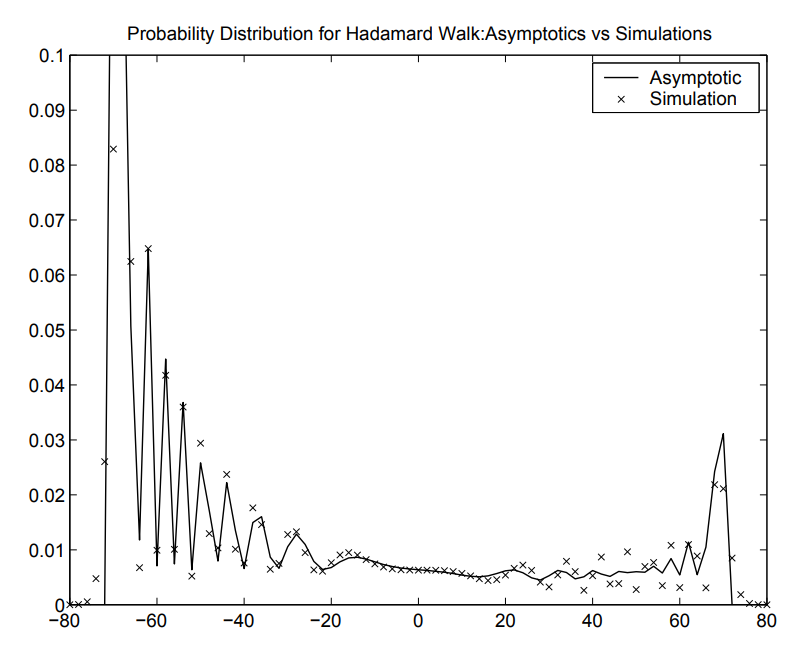
\includegraphics[width=1\textwidth]{Kap3/QWonlineNayak.png}
\caption{Simulación y función asintótica según la aproximación por el método de fase estacionaria, de una camianata con moneda de Hadamard y estado inicial $\ket{\downarrow,0}$, después de 100 pasos.}
\label{gr:Hadamard100Simulacion}
\end{figure}


\begin{table}[h]
    \centering
    \begin{tabular}{|c||c|c|c|c|c|c|c|c|c|c|c|c|}
        \hline
         &-5&-4&-3&-2&-1&0&1&2&3&4&5\\\hline\hline
        0&&&&&&1&&&&& \\ \hline
        1&&&&&$1/2$&&$1/2$&&&& \\\hline
        2&&&&$1/4$&&$1/2$&&$1/4$&&& \\ \hline
        3&&&$1/8$&&$5/8$&&$1/8$&&$1/8$&& \\ \hline
        4&&$1/16$&&$5/8$&&$1/8$&&$1/8$&&$1/16$& \\\hline
        5&$1/32$&&$17/32$&&$1/8$&&$1/8$&&$5/32$&&$1/32$ \\
    \hline
    \end{tabular}
    \medskip
    \caption{Las interferencias dan como resutado 
    probabilidades asimétricas alrededor de cero. Una mayor inteferencia negativa hace que el pico de la derecha sea menor que el de la iuerida, resultado de interferencias constructivas.}
    \label{TablaCuantica}
\end{table}
En las posiciones y tiempos $x+t$ impares la probabilidad es siempre nula, mientras que nunca lo es para $x+t$ par. La gráfica (\ref{gr:LineaHadamard100}) presenta la caminata en $t=100$ desde el estado inicial $\ket{\downarrow}\otimes\ket{0}$. 

\begin{figure}[ht]
\centering
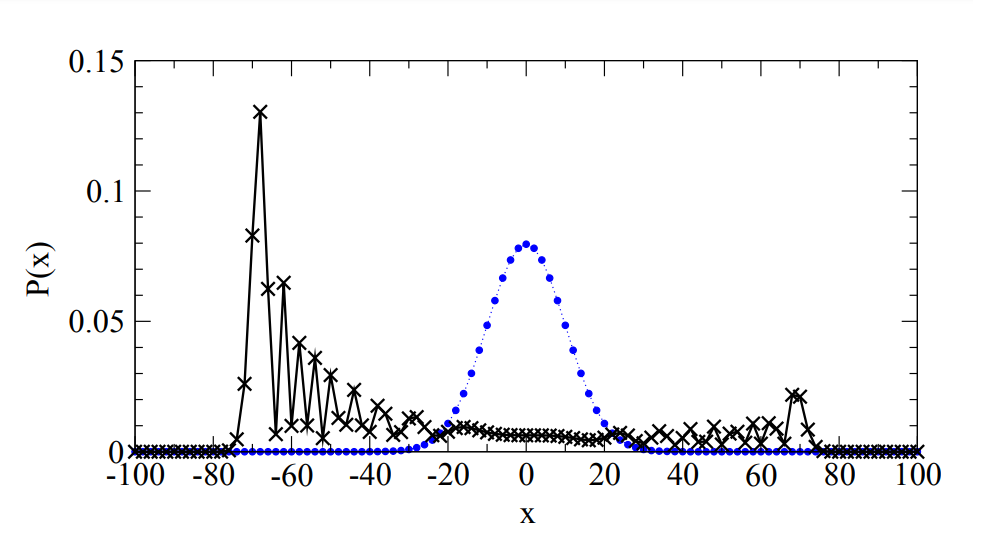
\includegraphics[width=1\textwidth]{Kap3/comparisonQW.png}
\caption{La distribución gaussiana de la caminata clásica y la distribución bimodal de la caminata cuántica con moneda de Hadamard y estado inicial $\ket{\downarrow,0}$, después de 100 pasos.}
\label{gr:LineaHadamard100}
\end{figure}

\subsubsection{Grados de libertad de la moneda}\label{sec:Moneda}
Hemos analizado la caminata lineal con la moneda balanceada de Hadamard, que, sin embargo, genera una caminata asimétrica. En esta sección comprobamos que la evolución de la caminata depende tanto de la moneda como de la condición inicial. Después se muestra que ambas condiciones son equivalentes.
El estado inicial $\ket{\psi_{\text{sim}}}=\frac{1}{\sqrt{2}}(\ket{0}+i\ket{1})\ket{x=0}$ hace simétrica la caminata con la moneda de Hadamard. La evolución para cada estado de la superposición es independiente debido a la fase $i$. Sin embargo, debido a que la probabilidad es independiente de la fase, el resultado final es la suma de dos distribuciones para dos caminatas independientes, la primera con sesgo hacia la izquierda (fase inicial $0$) y la otra hacia derecha (fase inicial $\pi$), que juntas hacen la gráfica simétrica \ref{gr:Hadamard100Symmetric}. \\

\begin{figure}[ht]
\centering
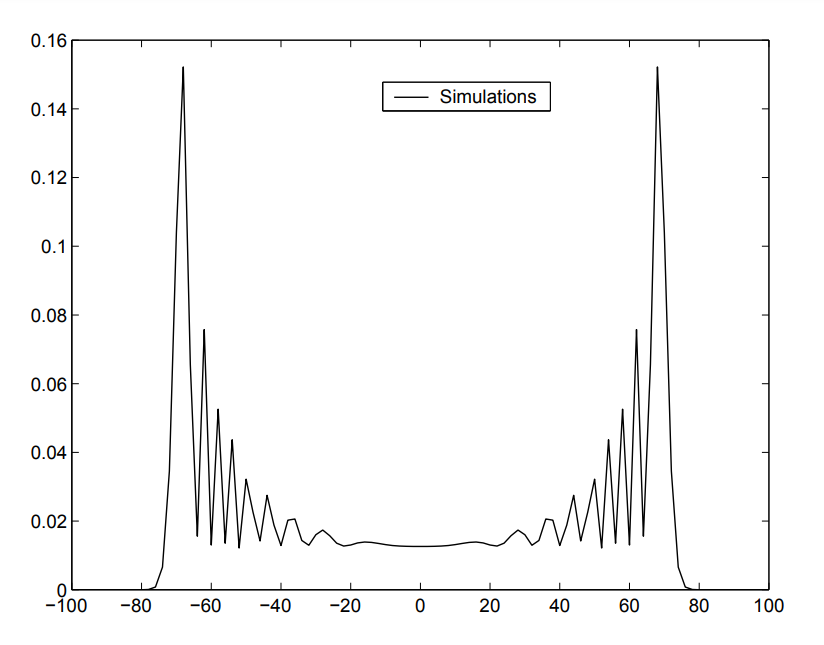
\includegraphics[width=1\textwidth]{Kap3/QWonlinesymmetricNayak.png}
\caption{Simulación de una camianata con moneda de Hadamard y estado inicial $\ket{\psi_{\text{sim}}}=\frac{1}{\sqrt{2}}(\ket{0}+i\ket{1})\ket{x=0}$, después de 100 pasos.}
\label{gr:Hadamard100Symmetric}
\end{figure}

La misma gráfica se obtiene si usamos el estado inicial hacia izquierda y la siguiente moneda balanceada diferente a la de Hadamard \cite{kempe2003quantum},
\begin{equation*}
\hat{Y}\doteq
\begin{pmatrix}
1 & i\\
i & 1
\end{pmatrix}
\end{equation*}{}
$\hat{Y}\ket{\uparrow}=\dfrac{1}{\sqrt{2}}(\ket{\uparrow}+i\ket{\downarrow})$, $\hat{Y}\ket{\downarrow}=\dfrac{1}{\sqrt{2}}(i\ket{\uparrow}+\ket{\downarrow})$.\\

$[$Bach, 2004$]$ muestra que la moneda más general es de la forma
\begin{equation}
    C_2^{(\text{gen})}=
    \begin{pmatrix}
    \sqrt{\rho}&\sqrt{1-\rho}e^{e\theta}\\
    \sqrt{1-\rho}e^{i\phi} & -\sqrt{\rho}e^{i(\theta+\phi)}
    \end{pmatrix}{},
    \label{MonedaGeneral}
\end{equation}{}
donde $0\leq\theta,\phi\leq\pi$ son ángulos arbitrarios, $0\leq\rho\leq1$.
Una moneda balanceada como la de Fourier y una no balanceada como la de Grover.
\begin{equation}
    \hat{\mathcal{F}} C_2^{(\text{gen})}=
    \begin{pmatrix}
    \sqrt{\rho}e^{-ik}&\sqrt{1-\rho}e^{i(-k+\theta)}\\
    \sqrt{1-\rho}e^{i(k+\phi)} & -\sqrt{\rho}e^{i(k+\theta+\phi)}
    \end{pmatrix}{},
    \label{MonedaGeneral}
\end{equation}{}

\subsection{Caminos con borde}
Los caminos con borde son otro ejemplo de la diferencia entre las caminatas aleatorias clásicas y cuánticas. Recortemos la línea infinita y ubiquemos una pared absorbente que termina la caminata cuando la partícula choca con ella. Llamemos $0$ a la posición de esta pared y asumamos que el camino inicia en $1$. En el caso clásico, todos las caminatas posibles chocan con la pared, ¡ninguna la evita!. Aunque la línea es infinita y la probabilidad de recorrerla siempre hacia la derecha es diferente de cero, el análisis indica que la partícula siempre retorna y choca en $0$. La siguiente demostración que se hace por recurrencia: sea $p_{10}$ la probabilidad de llegar a $0$ por \textit{cualquier} camino; en particular, sabemos que tras una iteración, la probabilidad de ir a $0$ desde $1$ es $1/2$, y un valor igual el de ir hasta $2$. Ahora nos interesa $p_{20}$ que es la probabilidad de ir a $0$ desde $2$ a lo largo de \textit{cualquier} camino. Notemos que $p_{20}=p_{21}p_{10}$.

\begin{equation}
p_{10}=\frac{1}{2}+\frac{1}{2}p_{21}p_{10} ,
\label{CaminataBorde}
\end{equation}{}
La homogeneidad del espacio hace equivalentes todos los caminos que tienen distancia uno hacia la izquierda, en particular $p_{21}=p_{10}=p$. Teniendo en cuenta esto, la ecuación (\ref{CaminataBorde}) tiene solución para $p=1$. 
\begin{equation}
p=\frac{1}{2}+\frac{1}{2}p^2 ,
\end{equation}
Esto es equivalente a afirmar que la caminata clásica es \textit{recurrente}, esto es, que la partícula pasa por (choca) cada punto de la recta infinitas veces.\\
En el caso cuántico el estado de posición es una superposición de las posiciones posibles. Para saber si la partícula fue absorbida en el punto $b$, se necesita hacer una medición $M_b$ en $b$ (en la pared absorbente), tras cada paso $\hat{U}$,

\begin{equation*}
    \hat{M}_b\ket{\psi}=
    \left\{
    \begin{array}{cl}
        \ket{b} & \qquad p_b=|\bra{b}\ket{\psi}|^2 \\
        \dfrac{\ket{\psi}-\braket{b|\psi}\ket{b}}{\sqrt{1-|\braket{b|\psi}|^2}} &\qquad p_{B_\perp}=1-|\braket{b|\psi}|^2 
    \end{array}
    \right.
\end{equation*}{}
Tras hacer una medición se anulan las correlaciones, que no se pueden recuperar ya que éste es un proceso irreversible. $M_b$ proyecta sobre dos subespacios, el punto $b$ solo, o su complemento. Si se encuentra la partícula en $b$ se deja de medir. [Kempe, 2003b] presenta dos protocolos útiles que llevan a la misma conclusión: ¡la partícula escapa con probabilidad $2/\pi$!
\chapter{Caminatas cuánticas sobre gráficas}

\section{Sobre el plano infinito}
Las caminatas sobre el plano infinito construido con rejilla cuadrada. Con tres monedas distintas la dispersión de

\subsubsection*{Grover}
\begin{equation}
H=\frac{1}{2}
\begin{pmatrix}
-1 & 1 & 1 & 1\\
1 & -1 & 1 & 1\\
1 & 1 & -1 & 1\\
1 & 1 & 1 & -1
\end{pmatrix}
\qquad ; \qquad    \ket{\Psi(0)}=\frac{1}{2}(\ket{00}-\ket{01}-\ket{10}+\ket{11})\otimes\ket{x=0,y=0}
\end{equation}{}

\begin{figure}[ht]
\caption{}
\centering
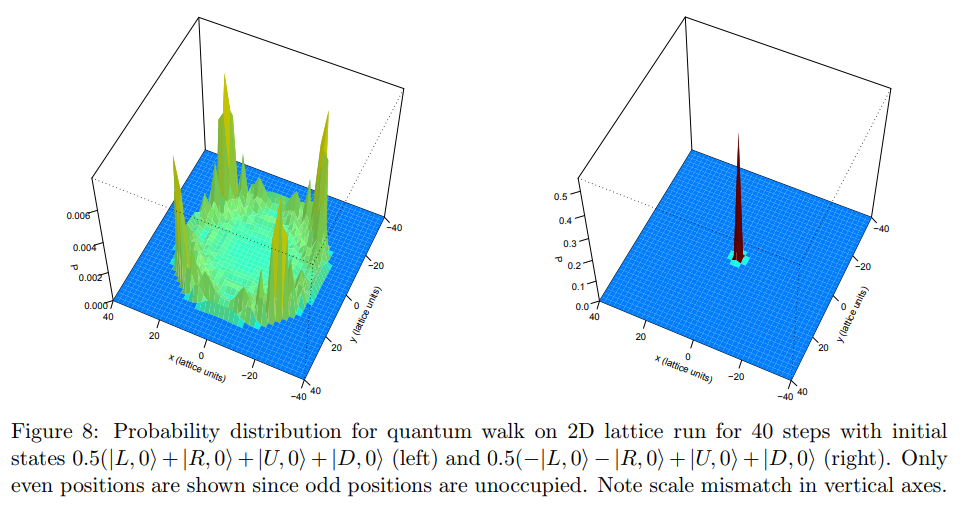
\includegraphics[width=0.5\textwidth]{QWGroverCoinKendonPercolation2019.png}
\end{figure}

\section{Gráficas finitas}
En el análisis de la dinámica definimos el \textit{periodo} y \textit{cuasi-periodo} de la distribución y damos las razones por las cuales no es posible converger a una distribución límite, a diferencia del caso clásico\cite{aharonov2001quantum}. Sin embargo, es usual el trabajo con una distribución promedio sobre las distribuciones originales que elimina la 'memoria' de los estados iniciales en el sistema permitiendo alcanzar una distribución estacionaria límite sobre esta nueva distribución. Introducimos los conceptos de \textit{mixing time} y \textit{hitting time} que descatan diferencias adicionales entre las caminatas, y más importante aún, descatan las ventajas (la mayoría de veces) de las caminatas cuánticas sobre las clásicas en la implementación de algoritmos.\\

El estudio sobre gráficas regulares finitas de clase 1 se puede generalizar a gráficas de clase 2 \cite{portugal2013quantum}.

\subsection{Definiciones básicas}

La evolución es la operación repetida de la moneda $\hat{C}$ y la traslación $\hat{S}$.
$\hat{U}=\hat{S}(\hat{C}\otimes I)$.
\begin{equation*}{}
\hat{S}\ket{j}\otimes\ket{v}=
    \left\{
    \begin{array}{cl}
    \ket{j}\otimes\ket{w}    & \text{if}\,\;\;\;\;e^j_v=(v,w) \\
    0  & \text{otherwise}
    \end{array}{}
    \right.
\end{equation*}{}
\subsection{Dinámica del sistema}

\noindent\textbf{Definición} Una caminata cuántica on base en la evolucíón por pasos $\ket{\psi(t)}=\hat{U}^t\ket{psi(0)}$ es \textit{periódica} si existe un \textit{periodo fundamental} $t_0\in\mathcal{Z}^+$ y un ángulo $\alpha$ tal que $\hat{U}^{t_0}=e^{i\alpha}\mathcal{I}$. Esto significa que $|\braket{\Psi(nt_0)|\Psi(0)}|^2=1$ para $n$ entero.\\

\noindent\textbf{Definición} Una caminata cuántica con base en la evolución $\ket{\psi(t)}=\hat{U}^t\ket{\psi(0)}$ tiene dinámica \textit{cuasi periódica} si para cualquier $\epsilon\in\mathbb{R}^+$, hay un tiempo $t$ tal que $||\hat{U}-\mathcal{I}||\leq\epsilon$.
Esto implica que para cualquier $\epsilon$ fijo, hay $t$ tal que $|\braket{\psi(t)|\psi(0)}|\geq1-\epsilon$.\\
En \cite{aharonov2001quantum} se lleva a cabo la estrategia para calcular la distribución límite para el N-círculo, equivalente para otras gráficas.\\
Dada la evolución unitaria de un sistema cuántico, siempre es posible su evolución contraria, porque a cada paso existe $\hat{U}^{-1}$ que revierte $\hat{U}$. Entonces la distribución después de muchos pasos depende de la estado inicial. Consideramos la distribución límite como la distribución uniforme sobre las distribuciones de probabilidad para cada estado inicial posible.\\

¿Existe el límite $\lim_{t\xrightarrow{}\infty}\ket{\psi(t)}$? Es posible una respuesta demostrando que la dinámica de las caminatas cuánticas sobre gráficas finitas es cuasi-periódica. Demos unas definiciones y el teorema correspondiente. "hay infinito número de tiempos een que el estado cuántico está cerca al estado inicial, presentando una estructura repetitiva en las escalas de tiempo."\\


\subsubsection{Algunas gráficas}

\subsubsection*{Ciclo}
Un N-ciclo tiene N vértices y condiciones de frontera periódicas, es decir, el vértices de los extremos coinciden y son el mismo. Un caminante sobre un vértices de un N-ciclo puede tomar dos direcciones: a favor o en contra de las manecillas del reloj. En el modelo de moneda, sus estados son $\{\ket{j,v}|j=0,1;v=0,\dots,N-1\}$.
\begin{equation}
    \hat{S}\ket{j,v}\xrightarrow{}\ket{j}\ket{j,v+(-1)^j}
\end{equation}{}
$v$ se incrementa si $j=0$. Usamos $\hat{H}$ para la evolución $\hat{U}=\hat{S}(\hat{H}\otimes I)$. Por la simetría espacial, la transformada de Fourier facilita la expresión que resulta de la operación de $\hat{U}$, en particular, los autoestados de $\hat{S}$
son los estados de la base ortnormal de Fourier $\{\widetilde{\ket{k}}|k\in [-\pi,\pi] \}$. Esto reduce el problema a diagonalizar $\hat{H}$, para obtener finalmente el espectro de la evolución:
\begin{equation}
    \hat{U}^t=\int_{-\pi}^\pi\frac{dk}{2\pi}\left(e^{-i\theta_kt}\ket{\alpha_k,\widetilde{k}}\bra{\alpha_k,\widetilde{k}}+e^{i(\pi+\theta_k)t}\ket{\beta_k,\widetilde{k}}\bra{\beta_k,\widetilde{k}}\right)
\end{equation}{}
Hallamos $\ket{\psi(t)}=\hat{U}^t\ket{\psi(0)}$ con la condición inicial $\ket{\psi(0)}=\ket{0}\ket{0}$, que es moneda a contrarreloj y posición del vértice $0$:

\begin{equation}
\ket{\psi(t)}=\dfrac{1}{N}    \sum_{j,k}A_k(t)e^{2\pi ikj/N}\ket{j}+\dfrac{1}{N}    \sum_{j,k}B_k(t)e^{2\pi ikj/N}\ket{j}
\end{equation}
donde $j$ y $k$ recorren todas las posiciones,

\begin{align}
    A_k=\cos\theta_k t-\dfrac{i\cos\kappa\sin\theta_kt}{\sqrt{1+\cos^2\kappa }}
    B_k=\dfrac{-ie^{i\kappa}\sin\theta_kt}{\sqrt{1+\cos^2\kappa}}
\end{align}
con $\kappa=2\pi k/N$. La probabilidad de estar en $j$ es

\begin{equation}
    P_j=\dfrac{1}{N}|\sum_{k}A_k(t)e^{2\pi ikj/N}|^2+\dfrac{1}{N}|\sum_{k}B_k(t)e^{2\pi ikj/N}|^2
\end{equation}
Estas ecuaciones son válidas para cualquier N, pero sólo para tiempos $t$ pares. Cuando $t$ es impar, intercambiamos $\cos\theta_k\xrightarrow{}-i\sin\theta_k$ en $A_k$ y $B_k$. 
En el N-ciclo los frentes de onda no se alejan siempre como en la línea infinita, por el contrario se acercan, y en $t\approx N/2$ se encuentran. Cuando $N$ es par las dos ondas interfieren sobre los puntos pares, en particular, en $N/2$. Por el contrario, para $N$ impar las ondas se entrecruzan en las posiciones, es decir, se dispersan sobre toda la gráfica pero sin tocarse, ya que para cualquier tiempo la posición de un frente son los impares mientras que para la otras son los pares. En tiempos grandes, para $N$ par y $t+j$ impar la probabilidad es nula, eso no es cierto en general para $N$ impar. Esta diferencia se evidencia mayormente en la distribución límite: que es uniforme e independiente para casos impares, y no uniforme y dependiente de las condiciones iniciales para ciclos pares.
Las interferencias introducidas a través de $\hat{H}$ no pueden ser reproducidas escogiendo adecuadamente las condiciones iniciales como en el caso de la línea infinita (ver sección (\ref{sec:Moneda})).\\

El periodo $T$ puede ser calculado a partir de $\hat{U}^T=I$, de lo cual se desprende que los autovalores de $\hat{U} $ a la potencia $T$ son $1$: $e^{-i\theta_k T}=e^{i(\pi+\theta_k)T}=1$ para todo $k$, cuyas soluciones más pequeñas son: $N=2,\, T=2$, $N=4,\,8$, $N=8,\,T=24$, $\dots$.

\begin{figure}[ht]
\centering
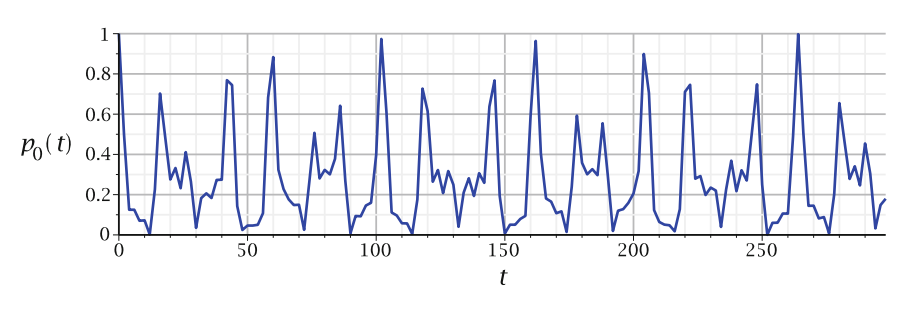
\includegraphics[width=0.8\textwidth]{Kap4/Quasiperiodyc10CyclePortugal.png}
\caption{Distribución del vértice $v=0$ en un 10-ciclo. En $t=264$ la probabilidad es muy cercana a $1$. Asimismo en otros tiempos la distribución es muy próxima a $1$.
\cite{portugal2013quantum}}
\end{figure}

\begin{equation}
    \Vec{c}^t=\frac{1}{t}\sum_{s=1}^t\Vec{p}^s
\end{equation}{}
\begin{equation}
c_i^t=\dfrac{1}{t}\sum_{s=1}^t\sum_{\alpha=\uparrow.\downarrow}\sum_{k,l=1}^{2N}a_ka_l*(\lambda_k\lambda_l*)^s\braket{\alpha,i|v_k}\braket{v_l|\alpha,i}
\end{equation}{}
\begin{equation}
    c_i^t\xrightarrow{t\xrightarrow{}\infty}\sum_{\alpha=\uparrow,\downarrow}\sum_{k,l=1}^{2N}a_ka_l^*\braket{\alpha,i|v_k}\braket{v_l|\alpha,i}=:\Vec{\pi_i}
\end{equation}{}


\subsubsection*{Gráfica 2D finita}
Una red 2D con condiciones de frontera periódicas corresponde a un \textit{toro}. Si la red tiene $N$ vértices, y sus lados $\sqrt{N}$, los estados en el modelo de moneda son $\{\ket{d,s}\otimes\ket{x,y}d,s=0,1,x,y=0,\dots \sqrt{N}-1\}$ en donde los estados de las monedas $\ket{d,s}$ están en $\mathcal{H}^2\otimes \mathcal{H}^2$, y son tales que $d$ designa el eje de movimiento: $d=0$ sobre el eje $x$, y $d=1$ sobre $y$, y si $s=0$ la dirección es hacia los negativos, y si $s=1$ hacia los positivos. Los estados de posición están en  $\mathcal{H}^{\sqrt{N}} \otimes   \mathcal{H}^{\sqrt{N}}$. La evolución $\hat{U}=\hat{S}\hat{C}$:

\begin{equation}
    \hat{S}\ket{d,s}\ket{x,y}\xrightarrow{}\ket{d,s}\ket{x+(-1)^{\delta_{0,s}},y+(-1)^{\delta_{1,s}}}
\end{equation}{}

\begin{equation}
    \ket{\psi(t)}=\dfrac{1}{\sqrt{N}}\ket{D}\ket{D}+\dfrac{1}{\sqrt{2N}}\sum_{\begin{array}{c} k,l=0\\ (k,l)\neq(0,0) \end{array}}^{\sqrt{N}-1} (e^{i\theta_klt}\ket{\nu_{kl}^{\theta}}+e^{-i\theta_klt}\ket{\nu_{kl}^{-\theta}})
\end{equation}
donde $\theta_{kl}=\frac{1}{2}(\cos{\dfrac{2\pi k}{\sqrt{N}}}+\cos{\dfrac{2\pi l}{\sqrt{N}}})$, y 
\begin{equation}
    \ket{\nu_{kl}^{\pm\theta}}=\dfrac{i}{2\sqrt{2}\sin{\theta_{kl}}}
      \left(
    \begin{array}{c}
        e^{i\theta_{kl}}-\omega^k   \\
        e^{-i\theta_{kl}}-\omega^{-k}\\
        e^{-i\theta_{kl}}-\omega^{l}\\
        e^{-i\theta_{kl}}-\omega^{-l}
    \end{array}
    \right)
\end{equation}
\subsubsection*{Hipercubo}
[17 en Kempe] Calculate the expected hitting time where an exponential speed up is reached. 
We have that the hypercube doesn't mixed at all in continuous quantum walk.
\cite{marquezino2008mixing}
\subsubsection*{Gráfica de árboles ligados}

\begin{figure}[ht]
\centering
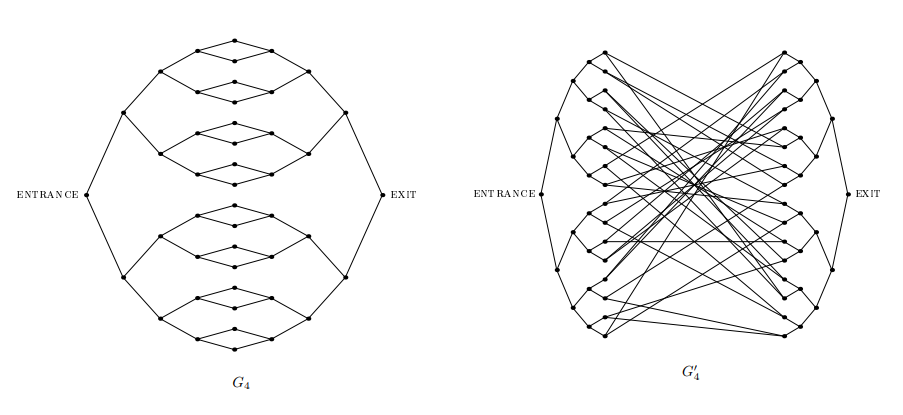
\includegraphics[width=1\textwidth]{Kap4/GluedTreesChilds.png}
\caption{La distancia de la mitad no es importante, sirve para esclarecer la imagen.  $G_n$ es más sencilla que $G_n'$.  \cite{childs2003exponential}}
\end{figure}

[Childs] [Fahri] analizaron la gráfica de árboles ligados con profundidad $n$, $G_n$, y compararon el \textit{hitting time} promedio con el caso clásico. Con la caminata en tiempo continuo obtuvieron una mejora en exponencial. 
\begin{figure}[ht]
\centering
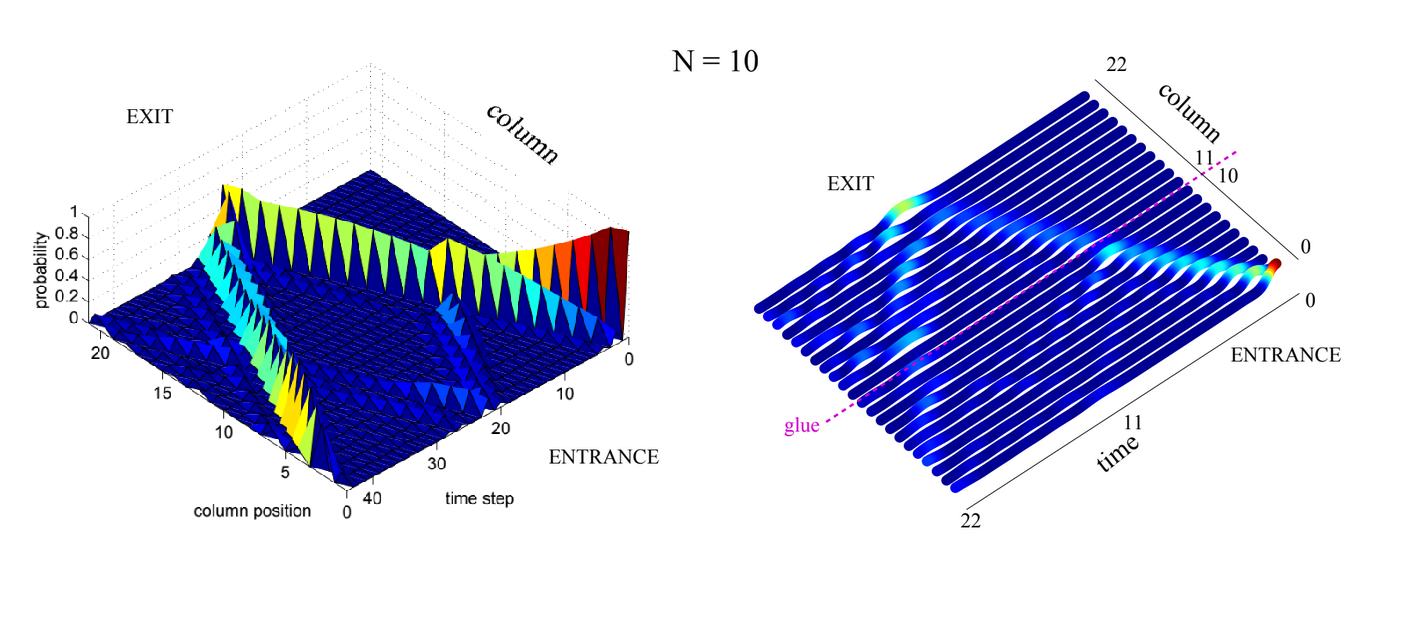
\includegraphics[width=1\textwidth]{Kap4/GluedTreesCarneiro.png}
\caption{Caminata de tiempo continuo en el que $G_4$, para $N=10$. \cite{carneiro2005entanglement}}
\end{figure}

\begin{equation*}
    \ket{\text{col}\,j}=\dfrac{1}{\sqrt{N_j}}\sum_{v\,\in \, \text{column}\,j} \ket{v},
\end{equation*}{}

where

\begin{equation*}
    N_j=
    \left\{
    \begin{array}{ll}
    2^j & 0\leq j\leq n\\
    2^{2n+1-j} & n+1\leq j \leq 2n+1
    \end{array}
    \right.
\end{equation*}{}
\begin{equation*}
    \bra{\text{col}\,j}H\ket{\text{col}\,(j+1)}=
    \left\{
    \begin{array}{ll}
    \sqrt{2}\gamma     & 0\leq j\leq n-1\,,\,\,\,n+1\leq j\leq 2n  \\
    2\gamma     & j=n 
    \end{array}{}
    \right.
\end{equation*}{}

\begin{equation*}
    \braket{j|p}=\dfrac{1}{\sqrt{2\pi}}e^{ipj},\,\,\,\,\,\,-\pi\leq p\leq\pi
\end{equation*}{}
having energies $E_p=2\cos p$
\begin{align*}
    G(j,k,t)&=\bra{k}e^{-i\hat{H}t}\ket{j}\\
    &=\dfrac{1}{2\pi}\int_{-\pi}^{\pi}dp e^{ip(k-j)-2it\cos p}\\
    &=(-i)^{k-j}J_{k-j}(2t), \,\,\,\,\,\, -\infty < j,k < \infty
\end{align*}{}

\begin{align}
    J_\nu(\nu/\cosh{\zeta})
\end{align}{}

La probabilidad de estar en la raíz derecha habiendo partido de la raíz izquierda es:
\begin{equation}
    \Vec{\pi}\geq \frac{1}{2n+1},
\end{equation}
por su parte en el caso clásico:
\begin{align}
    \pi_b&=\lim_{t\xrightarrow{}\infty} p_b(t),
    \pi_b&=(2^{n+1}+2^n-2)^{-1}\\
\end{align}
\cite{childs2002example}


%\begin{figure}[ht]
%\caption{addfad}
%\centering
%\includegraphics[width=0.5\textwidth]{.png}
%\end{figure}


\section{Algoritmos con base en caminatas cuánticas}
Empezando por el algoritmo de Shor para la factorización, los primeros algoritmos se basaban en la transformada de fourier para poder identificar un subgrupo escondido (Lomont 2004). En los límites de este método se plantea la pregunta sobre otros posibles métodos eficientes, y una de las búsquedas se lleva a cabo en la correspondiente cuántica al área exitosa de las caminatas aleatorias.
En esta sección mencionamos algunos problemas de la computación para los cuales existe un algoritmo basado en una caminata cuántica que lo soluciona.\\

Iniciamos con el problema de atravesar la \textit{gráfica de árboles ligados} $G_n$, cuyo algoritmo fue el primero que incluyó una caminata cuántica con una mejora exponencial respecto de la clásica, en el marco del oráculo. En la sección anterior mostramos su dinámica, ahora cómo es posible aplicarla en un algoritmo. Esto nos sirve para presentar el concepto del \textit{oráculo}, en el que se basa el marco de comparación de eficiencia llamado \textit{complejidad de consultas}.\\

El algoritmo de Ambainis \cite{ambainis2007quantum} para resolver el problema de los elementos distintos en un conjunto sirve como base para implementación de otros algoritmos. Finalmente, el problema de la búsqueda espacial ha tenido diferentes soluciones. El esquema de búsqueda de Szegedy \cite{szegedy2004quantum} basado en la cuantización de la caminata, y las mejoras de Magníez et al. \cite{magniez2011search} son importantes. Un ejemplo de búsqueda espacial es sobre una base de datos física.\\

Los algoritmos se presentan con base en la estructura de \cite{shao}.
\subsection{Atravesar la gráfica de árboles ligados}
Childs et al. \cite{childs2003exponential} fueron los primeros en presentar un algoritmo basado en una caminata cuántica exponencialmente más rápido que el clásico. Para ello solucionaron el problema de atravesar la gráfica $G_n'$ desde un vértice extremo hasta el opuesto. Es un problema poco práctico pero que muestra el poder de las caminatas cuánticas. En el mismo trabajo presentaron la implementación el algoritmo como la simulación de un hamiltoniano correspondiente. \\ 

El problema es el siguiente:\\

\textit{Dado un oráculo de la gŕafica $G_n$, y partiendo del vértice ENTRADA, ¿cuántos pasos cuesta llegar al vértica SALIDA?}\\

Los vértices reciben nombres aleatoriamente. El oráculo de la gráfica da los nombres de los vértices vecinos al que le ingresamos. Describamos primero la solución En el marco del oráculo se tiene el siguiente algoritmo clásico óptimo, no basado en una caminata aleatoria, que toma $\mathcal{O}(t^2)$. Partiendo de ENTRADA.
\begin{center}
    \begin{tabular}{l}
    \hline \textbf{Algoritmo para cruzar $G_n$} \\\hline 
    \textbf{1.} 
    \\\hline
    \end{tabular}{}
\end{center}{}

La implementación como algoritmo:
\subsection{Algoritmo de elemento distinto de Ambainis}
Los siguientes son problemas importantes solucionados con caminatas cuánticas sobre gráficas adecuadas[design,2019]:
\begin{itemize}
\item graph collision problem,
\item single source shortest path,
\item search on the grid(65-68[design]),
\item NAND true evaluation
\item forbidden subgraph propierty
\item tringle finding,
\item subset sum problem,
\item element distinctness problem,
\item group commutativity test,
\item matrix product verification,
\item Boolean matrix multiplication,
\item algebraic property test,
\end{itemize}{}

\subsection{Búsqueda espacial}

El problema de búsqueda espacial es el siguiente:\\

\textit{Dada una gráfica, ¿cuántos pasos cuesta encontrar 1 o más elementos  marcados?}\\

\noindent Un algoritmo de búsqueda típico se desarrolla en tres pasos: la etapa de preparación, la actualización y el chequeo.
\begin{enumerate}
    \item $[$Preparar$]$ Acceder a algún estado de $\Gamma$, usualmente un estado aleatorio o uno de superposición uniforme en el caso cuántico,
    \item $[$Actualizar$]$ llevar de un estado a otro estado con una caminata aleatoria (clásica o cuántica), y
    \item $[$Chequear$]$ chequear durante la caminata para saber si el estado actual está marcado.
\end{enumerate}
"El algoritmo debe ser local sobre la gráfica." Childs.

\begin{center}
    \begin{tabular}{l}
    \hline \textbf{Algoritmo de búsqueda clásico} por 1 paso de caminata aleatoria\\\hline 
    \textbf{1.} [Preparar] Obtener de $\Gamma$ un vértice $u$.\\
    \textbf{2.} Realizar lo siguiente $h=\mathcal{O}(1/(\epsilon \delta))$ número de veces, de acuerdo a la estimación [(5.11) Shao]:\\
    2.1 [Chequear] Si $u$ está marcado, retornar $u$ y  parar.\\
    2.2. [Actualizar] Empezar desde $u$, simular una caminata aleatoria $P$ en $\Omega$ en un paso.\\
    \textbf{3.} Retornar "no ítem marcado"\\\hline
    \end{tabular}{}
\end{center}{}

\begin{center}
    \begin{tabular}{l}
    \hline \textbf{Algoritmo de búsqueda clásico} por multipasos de caminata aleatoria\\\hline 
    \textbf{1.} [Preparar] Obtener de $\Gamma$ un vértice $u$.\\
    \textbf{2.} Realizar lo siguiente $h(\pi^T,\mathcal{M})=\mathcal{O}(1/(\epsilon ))$ número de veces (que es el \textit{hitting time} promedio desde \\la distribución estacionaria en $\Gamma$:\\
    2.1 [Chequear] Si $u$ está marcado, retornar $u$ y  parar.\\
    2.2. [Actualizar] Empezar desde $u$, simular una caminata aleatoria $P$ en $\Omega$ durante $T_{\text{mix}}=\mathcal{O}(1/\delta)$ pasos\\ (hasta alcanzar la distribución estacionaria $\pi^T$).\\
    \textbf{3.} Retornar "no ítem marcado"\\\hline
    \end{tabular}{}
\end{center}{}

\subsubsection{Algoritmos de búsqueda sobre gráficas finitas}
La idea de Benioff [Cite Benioff 2002] fue pionera en la  búsqueda espacial asociando a una región finita del espacio una gráfica sobre cuyos vértices se para un \textit{robot cuántico}, y sobre cuyas aristas camina.
Una búsqueda clásica corresponde a tomar aleatoriamente un vértice de la gráfica, lanzar una moneda de dimensión igual al grado del vértice, y moverse a lo largo de la arista etiquetada hasta llegar a nuevo vértice. El caminante repite el proceso aleatorio sin memoria del camino ni clave para encontrar el objetivo, que sólo alcanza cuando se para sobre el vértice marcado.\\

Presentamos los casos cuánticos de la red finita en 2D con condiciones de frontera periódicos (que es un \textit{toro}) y el hipercubo que usan los resultados encontrados arriba.\\
La idea consiste en usar el operador de difusión de Grover $\hat{R}=2\sum_{v\in \mathcal{M}}\ket{v}\bra{v}-I$  (ver apéndice (\ref{sec:Grover})) en cada iteración, intercalado con la caminata usual sobre la gráfica. El resultado final depende altamente de la distribución de los elementos marcados sobre la gráfica cuando $|\mathcal{M}|>1$, así que evaluamos el caso en que hay un solo elemento marcado. En ese caso, $R=2\ket{0}\ket{0}-I$, donde llamamos $0$ al vértice marcado.
\noindent El operador de búsqueda es $\hat{U'}=\hat{U}\hat{R}$. De $\hat{U'}$, sean los autovalores $\{e^{i\lambda_1},\dots, e^{i\lambda_k}\}$. Para la mayor parte de las gráficas, los autovalores $\lambda$ y $\lambda'$ corresponden a los autovalores  prevalentes de $\hat{U'}$ para tiempos largos (no presentamos demostración), (ver gráfica \ref{gr:EspectroBusqueda}). Los respectivos autovectores son $\ket{\lambda}$ y $\ket{\lambda'}$. $\lambda=\lambda'$ para muchas gráficas. Lo anterior nos permite escribir:

\begin{figure}[ht]
\centering
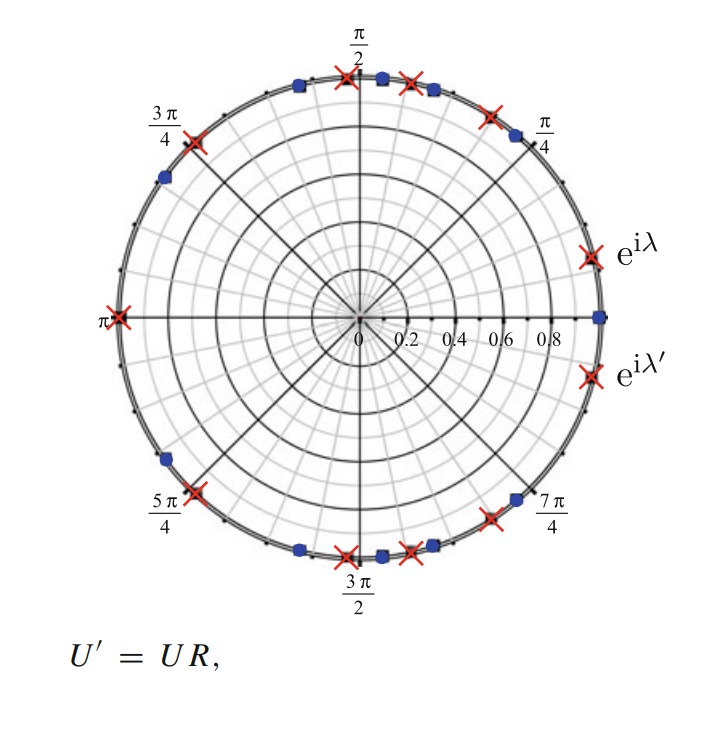
\includegraphics[width=0.5\textwidth]{Kap5/SpatialSearchUprimePortugal.png}
\caption{Autovalores de $\hat{U}$ y $\hat{U'}$. El de argumento menor positivo $e^{i\lambda}$ y el de mayor negativo $e^{-i\lambda'}$ están señalados. Para $t$ muy grandes $\lambda$ y $\lambda'$ tienden a 1, y son los únicos relevantes para la dinámica.
\cite{portugal2013quantum}}
\label{gr:EspectroBusqueda}
\end{figure}

\begin{equation}
    \hat{U}^t=e^{i\lambda t}\ket{\lambda}\bra{\lambda}+e^{i\lambda't}\ket{ \lambda'}\bra{\lambda'}+\hat{U}_{\text{small}}^t
\end{equation}{}
$\hat{U'}$ actúa no trivialmente sobre el subespacio ortogonal al generado por los otros dos, $\{\ket{\lambda},\ket{\lambda'}\}^{\perp}$

\begin{equation}
    p(t)=|e^{i\lambda t}\braket{0|\lambda}\braket{\lambda|\psi(0)}+e^{i\lambda't}\braket{0|\lambda'}\braket{\lambda'|\psi(0)}+\epsilon|^2
    \label{ec:ProbEigenphaseDeco}\,\qquad\text{donde}\,\,\epsilon=\braket{0|\hat{U}^t_{\text{small}}|\psi(0)}
\end{equation}

Se puede demostrar para ciertas gráficas que $\lim_{N\xrightarrow{}\infty}\epsilon=0$. Resta encontrar $\lambda$, $\lambda'$, $\braket{0|\lambda}$, $\braket{0|\lambda'}$, y $\braket{\lambda|\psi(0)}$, $\braket{\lambda'|\psi(0)}$. Encontramos los resultados para $\lambda$, los correspondientes de $\lambda'$ tienen un desarrollo análogo. Llevamos a cabo el objetivo asumiendo la descomposición espectral de $\hat
{U}$: $\hat{U}\ket{\psi_k}=e^{i\phi_k}\ket{\psi_k}$.
Encontramos $\lambda$ resolviendo $A-B\lambda$-C$\lambda^2$=$\mathcal{O}(\lambda^3)$, con
\begin{align}
    A&=2\sum_{\phi_k=0}|\braket{0|\psi_k}|^2,\\
    B&=\sum_{\phi_k\neq0}\dfrac{|\braket{0|\psi_k}|^2\sin{\phi_k}}{1-\cos\phi_k},\\
    C&=\sum_{\phi_k\neq0}\dfrac{|\braket{0|\psi_k}|^2}{1-\cos\phi_k}.\\
\end{align}
Además,
\begin{align}
    \braket{0|\lambda}&=\dfrac{|\lambda|}{\sqrt{2}\sqrt{A+C\lambda ^2}}+\mathcal{O}(\lambda),\,\,\text{y}\\
    \braket{\psi(0)|\lambda}&=\braket{\psi(0)|0}\braket{0|\lambda}\Big(1+\frac{i\sin\lambda}{1-\cos\lambda}\Big)
\end{align}
Se puede demostrar que existe uno y sólo un autovalor $\lambda$. Si los autovalores de $\hat{U}$ vienen en pares complejos conjugados $e^{i\phi_k}$, y $e^{-i\phi_k}$, $B=0$, pues contiene $\sin\phi_k$ que es antisimétrica. En tal caso:

\begin{align}
    \lambda&=-\lambda'=\sqrt{\frac{A}{C}},\\
    \braket{0|\lambda}&=\braket{0|\lambda'}=\frac{1}{2\sqrt{C}},\\
    \braket{\psi(0)|\lambda}&=\braket{\psi(0)|0}\Big( \frac{1}{2\sqrt{C}}+\frac{i}{\sqrt{A}}\Big).
\end{align}
La probabilidad (\ref{ec:ProbEigenphaseDeco}):
\begin{equation}
    p(t)=\frac{|\braket{\psi(0)|0}|^2}{AC}\sin^2\lambda t
\end{equation}
de lo cual se tiene que $t_{\text{opt}}=\lfloor\frac{\pi}{2\lambda}\rfloor$, y $p_{\text{success}}(t)=\dfrac{|\braket{\psi(0)|0}|^2}{AC}$

\subsubsection*{Gráfica 2D finita}
\begin{align}
    t_{\text{opt}}&=\lfloor\frac{\pi \sqrt{C}\sqrt{N\ln N}}{2\sqrt{2}}\rfloor\\
    p_{\text{success}}&=\frac{1}{2C\ln N}+\mathcal{O}^{-N}
\end{align}
$\hat{U'}$ se puede expresar como $\hat{U'}=\hat{S}\hat{C'}$, que es una caminata cuántica en el modelo de moneda con dos particularidades: $\hat{S}$ es una moneda \textit{flip-flop}, que opera trasladando, y además cambia el estado de moneda al valor contrario. Por su parte, $\hat{C'}$ es una moneda inhomogenea dependiente de la posición.
\subsubsection*{Hipercubo}
\begin{align}
    t_{\text{opt}}&=\lfloor\frac{\pi \sqrt{CN}}{4}\rfloor\\
    p_{\text{success}}&=\frac{1}{C}+\mathcal{N^{-1}}.
\end{align}
Esta búsqueda sobre el hipercubo basada en una caminata cuántica iguala la cota inferior del algoritmo de Grover.
Esta búsqeuda también se puede expresar como $\hat{U'}=\hat{S}\hat{C'}$.\\
\cite{shenvi2003quantum} \cite{ambainis2003quantum} Ambainis, 2003.
\begin{center}
    \begin{tabular}{l}
    \hline \textbf{Búsqueda en un hipercubo} \\\hline 
    \textbf{1.} [Preparar] Preparar el estado inicial $\ket{\psi}$:\\ $\ket{\psi}=\dfrac{1}{\sqrt{Nn}}\sum_{x,i}\ket{x}\ket{i}$\\
    \textbf{2.} Realizar lo siguiente $\mathcal{O}(\sqrt{N})$ número de veces:\\
    2.1. [Chequear y lanzar la moneda] Si $x$ no está marcado aplicar $R$ al registro $\ket{i}$,\\
    sino aplicar $-\mathbb{I}$ al registro $\ket{i}$\\
    2.2. [Actualizar] Aplicar $S:\ket{x}\ket{i}\xrightarrow{}\ket{\text{flip}(x,i)}\ket{i}$\\
    \textbf{3.} Medir el estado final del primero registro ($\ket{x}$).\\\hline
    \end{tabular}{}
\end{center}{}



Trabajos posteriores modifican su método mejorando la eficiencia [Tulsi], [Ambainis]

\subsection{Otros marcos de búsqueda espacial}
\cite{magniez2011search} Magniez, 2011,
\cite{szegedy2004quantum} Szegedy presented a speed up for markov chains based algorithms. \\
Este es un ejemplo, \\
Loke, Wang\\

\begin{center}
    \begin{tabular}{l}
    \hline \textbf{Algoritmo de Szegedy} para detectar \textbf{si $|\mathcal{M}|=0$}\\\hline 
    \textbf{1.} Preparar el estado inicial $\ket{\pi}$:\\
    $\ket{\pi}=$\\
    \textbf{2.} Aplicar $\mathcal{O}(\sqrt{h})$ número de veces la siguiente caminata:\\
    $[$Chequeo y actualización simultáneas$]$ $W(P_M)$\\
    \textbf{3.} Construir el siguiente estado:\\
    $\frac{1}{2}\ket{0}(\ket{\pi}+(W(P_M))^t\ket{\pi})+\frac{1}{2}\ket{1}(\ket{\pi}-(W(P_M))^t\ket{\pi})$\\
    \textbf{4.} Medir el estado final en el registro de control.\\\hline
    \end{tabular}{}
\end{center}{}

Una aplicación interesante de estas caminatas se da en la memoria \textit{ECM} de un agente de aprendizaje por refuerzo llamado \textit{PS-agent} o agente de simulación proyectiva \cite{briegel2012projective}. Un agente de esta clase toma decisiones sobre sus acciones de acuerdo a la información que percibe del ambiente, bajo un marco llamado procesos de decisión de Markov. La ECM es un grafo dirigido en el cual los vértices son los posibles estados y acciones, algunos de los cuales se conectan por aristas que pueden contener refuerzos positivos o negativos, que generan preferencias sobre los caminos, es decir, cambios en las parejas estado-acción, que finalmente conduce al agente al aprendizaje de alguna conducta. 
[Paparo et al, 2014]  presenta una modificación del protocolo sobre el proceso de decisión del agente, basado en las caminatas cuánticas en el marco de Szegedy, y demuestra que efectivamente la velocidad del proceso mejora cuadráticamente como se espera, y además demuestra que el las características del aprendizaje del agente bajo ambos protocolos es el mismo (que es mensurable en las probabilidades de las acciones que generan). Esto es importante porque las características prácticas y exitosas del aprendizaje del agente no cambian. Un cambio en la demora de la decisión puede ser determinante en ambientes que cambian en tiempos del mismo orden de magnitud.


\begin{center}
    \begin{tabular}{l}
    \hline \textbf{Marco de caminata cuántica MNRS} \\\hline 
    \textbf{1.} Preparar el estado inicial $\ket{\pi}$:\\
    $\ket{\pi}=\sum_{u\in G}\sqrt{\pi_u}\ket{u}\ket{p_u}=\sqrt{\sum_{u\in M}\pi_u}\ket{\pi_{\text{good}}}+\sqrt{\sum_{u\nin M}\pi_u}\ket{\pi_{\text{good}}}$\\
    \textbf{2.} Realizar lo siguiente $\mathcal{O}(1/\sqrt{\epsilon})$  número de veces:\\
    2.1. $[$Chequear$]$ Hacer la reflexión $R_{\ket{\pi_{\text{bad}}}}$ con respecto a $\ket{\pi_{bad}}$\\
    2.2. $[$Actualizar$]$ Hacer la reflexión $R_{\pi}$ con respecto a $\ket{\pi}$.\\
    \textbf{3.} Medir el estado final.\\\hline
    \end{tabular}{}
\end{center}{}
\begin{table}[h]
    \centering
    \begin{tabular}{|c|c|c|}
    \hline  
    Algoritmo & Costo para el caso $|\mathcal{M}|=1$ & Costo para el caso $\mathcal{M}>1$ \\\hline\hline
    Szegedy\cite{szegedy2004quantum} (2004)& $\sqrt{\frac{h}{N}}(S+\sqrt{h}(U+C))$ & $-$ \\\hline   
    MNRS (2011)&$S+\frac{1}{\sqrt{\epsilon}}(\frac{1}{\sqrt{\delta}}U+C)$ & $S+\frac{1}{\sqrt{\epsilon}}(\frac{1}{\sqrt{\epsilon}}U+C)$ \\\hline
    Magniez, et al (2012) & $S+\sqrt{h}(U+C)$ & $-$\\\hline
    Krovi, et al. (2016)& $S+\sqrt{h}(U+C)$&$S+\sqrt{h^+}(U+C)$
    \\\hline
    Dohotaru and Hoyer (2017)&$S+\sqrt{h}U+\frac{1}{\sqrt{\epsilon}}C$&$S+\sqrt{h^+}(U+C)$\\\hline
    \end{tabular}
    \caption{\cite{shao}}
    \label{AlgoritmosBusqueda}
\end{table}{}

\subsubsection*{Árbol de hexágonos}
En este caso no presentamos desarrollos analíticos sino los resultados de implementaciones experimentales. 

\begin{figure}[ht]
\centering
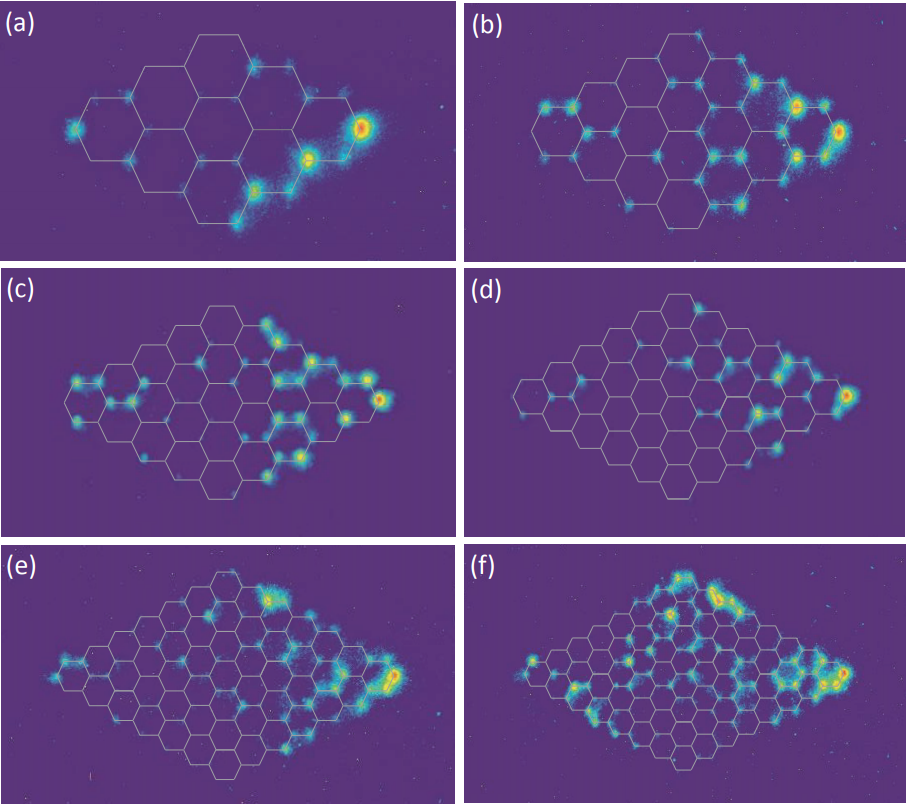
\includegraphics[width=0.7\textwidth]{Kap5/HexagonWalkTang2018.png}
\caption{Experimental }
\end{figure}

\chapter{Conclusiones y recomendaciones}
\section{Conclusiones}
La aleatoriedad aparece 


Las conclusiones constituyen un cap\'{\i}tulo independiente y presentan, en forma l\'{o}gica, los resultados de la tesis  o trabajo de investigaci\'{o}n. Las conclusiones deben ser la respuesta a los objetivos o prop\'{o}sitos planteados. Se deben titular con la palabra conclusiones en el mismo formato de los t\'{\i}tulos de los cap\'{\i}tulos anteriores (T\'{\i}tulos primer nivel), precedida por el numeral correspondiente (seg\'{u}n la presente plantilla).\\

\section{Recomendaciones}
Se presentan como una serie de aspectos que se podr\'{\i}an realizar en un futuro para emprender investigaciones similares o fortalecer la investigaci\'{o}n realizada. Deben contemplar las perspectivas de la investigaci\'{o}n, las cuales son sugerencias, proyecciones o alternativas que se presentan para modificar, cambiar o incidir sobre una situaci\'{o}n espec\'{\i}fica o una problem\'{a}tica encontrada. Pueden presentarse como un texto con caracter\'{\i}sticas argumentativas, resultado de una reflexi\'{o}n acerca de la tesis o trabajo de investigaci\'{o}n.\\
\begin{appendix}
\chapter{Algoritmo de Grover}\label{sec:Grover}

El algoritmo de Grover es el algoritmo cuántico de búsqueda óptimo en un conjunto desordenado \cite{grover1996fast}, \cite{nielsen2002quantum}. Lo llevamos a cabo con el operador de Grover $\hat{G}$ que es producto de dos operaciones en el espacio de n qubits $\hat{G}=(2\ket{\psi}\bra{\psi}-I)\hat{O}$: (1) el operador $\hat{O}:\ket{x}\xrightarrow{}(-1)^{f(x)}\ket{x}$, donde $f(x)$ es la función oráculo que tiene valor $f(x)=0$ cuando $x$ no es respuesta a la consulta (no es el elemento marcado), y $f(x)=1$ cuando $x$ sí es respuesta. $\hat{O}$ aplica un cambio de fase sobre los elementos marcados del conjunto. (2) el operador $2\ket{\psi}\bra{\psi}-I$ denomiado difusor de Grover.
\begin{equation}
\ket{\psi}=\hat{H}^{\otimes n}\ket{0}=\frac{1}{\sqrt{N}}\sum_{x=0}^{N-1}\ket{x}
\end{equation}
\noindent Es posible un mapeo del espacio de Hilbert de los n qubits sobre los subespacios $\ket{\alpha}$, superposición de los elementos no marcados, y $\ket{\beta}$, superposición de los marcados, es decir $\mathbb{R}^2$, cuyo producto tensorial genera un subespacio en el que $\ket{\psi}$ y $\hat{G}\ket{\psi}$ están contenidos. Ver la gráfica (\ref{gr:Grover}).

\begin{equation}
    \ket{\alpha}=\frac{1}{\sqrt{N-M}}\sum_x\,^{'}\ket{x}\qquad,\qquad    \ket{\beta}=\frac{1}{\sqrt{M}}\sum_x\,^{''}\ket{x}
\end{equation}
$\ket{\psi}$ como combinación de $\ket{\alpha}$ y $\ket{\beta}$ es:
\begin{equation}
\ket{\psi}=\sqrt{\dfrac{N-M}{N}}\ket{\alpha}+\sqrt{\dfrac{M}{N}}\ket{\beta}
\label{ec:GroverInicial}
\end{equation}{}
La aplicación de $\hat{O}$ genera un reflexión alrededor de $\ket{\alpha}$, y $(2\ket{\psi}\bra{\psi}-I)$ una reflexión alrededor de $\ket{\psi}$. Ambas reflexiones generan una rotación como en la gráfica. Llamemos $\cos{\theta/2}=\sqrt{(N-M)/N}$, y $\sin{\theta/2}=\sqrt{M/N}$. La rotación tras una aplicación es $\theta$:

\begin{equation}
    \hat{G}\ket{\psi}=\cos\frac{3\theta}{2}\ket{\alpha}+\sin\frac{3\theta}{2}\ket{\beta}
\end{equation}
En efecto, $\hat{G}$ tiene la representación de una rotación usual en $\mathbb{R}^2$ (como en \ref{MatrizRotaciones}).\\
Si rotamos las veces necesarias hasta estar muy próximos al estado $\ket{\beta}$, una medición tendrá alta probabilidad de resultar en un elemento marcado.
¿Cuántas veces debe operar $\hat{G}$ para que el vector final sea tan próximo a $\ket{\beta}$? Para responder, notemos el ángulo complementario a $\theta/2$: $\arccos\sqrt{M/N}$, entonces la cantidad de rotaciones apropiada es:
\begin{equation}
    R=\text{CI}\big( \dfrac{\arccos\sqrt{M/N}}{\theta}\big)
    \label{ec:RGrover}
\end{equation}

\begin{figure}[ht]
\centering
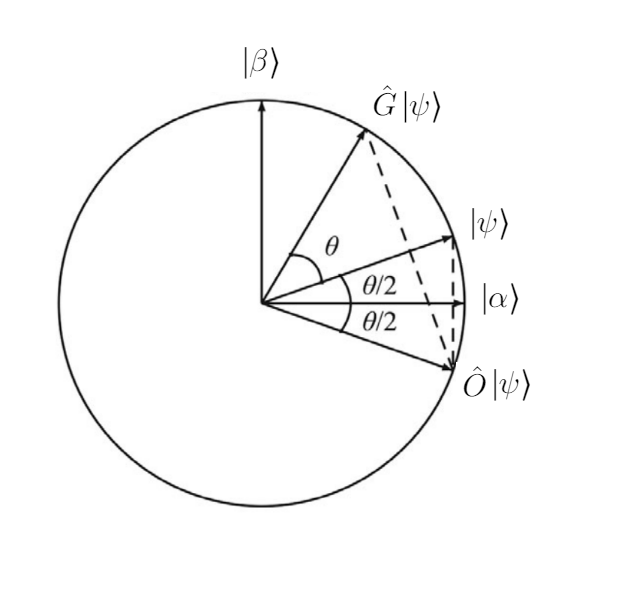
\includegraphics[width=0.6\textwidth]{Anexos/grover.png}
\caption{Grover}
\label{gr:Grover}
\end{figure}
donde $\text{CI}(x)$ es el entero completo de $x$, por ejemplo $\text{CI}(3,72)=3$. Tras aplicar $R$ veces el operador de Grover, el ángulo final sobre $\ket{\beta}$ es $<\pi/4$ y la probabilidad de medir un elemento marcado es significativa, $\pi^2/16>1/2$. El caso particular $M\ll N$ es notorio: $\theta/2\approx \sin(\theta/2)\approx \sqrt{M/N}$, con lo cual $R\approx N/M$, y el error después de la medición es $M/N$. \\
La complejidad del algoritmo es igual al número de rotaciones $R$, ya que cada aplicación tiene el costo de un solo llamado al oráculo. en (\ref{ec:RGrover}) $R$ tiene una cota superior $R=\lceil\pi/2\theta \rceil$, debido al máximo valor posible del numerador. Ahora, una cota inferior de $\theta$ impone otra cota superior sobre $R$.

\begin{equation}
    \frac{\theta}{2}>\sin\frac{\theta}{2}=\sqrt{\frac{M}{N}}
\end{equation}
Así que $R=\mathcal{O}(\frac{\pi}{4}\sqrt{\frac{N}{M}})$

Así que $R=\mathcal{O}(\sqrt{N/M})$ y en el caso de $M=1$, $R=\mathcal{O}(\sqrt{N})$.

\begin{center}
    \begin{tabular}{l}
    \hline \textbf{Algoritmo de Grover}\\\hline
    \textbf{entradas:} \\
    \textbf{salidas:}\\\hline
    \textbf{proceso}\\
    \textbf{1.} [Preparar:] Preparar el estado inicial $\ket{\psi}$ como en (\ref{ec:GroverInicial}).\\
\textbf{2.} Ejecutar lo siguiente $\mathcal{O}(\sqrt{N/M})$ número de veces:\\
(a) [Chequear:] Aplicar $\mathcal{O}$ (reflexión con respecto a $\ket{\alpha}$)\\
(b) [Actualizar:] Aplicar $2\ket{\psi}\bra{\psi}-I$ (reflexión con respecto a $\ket{\psi}$)\\
\textbf{3.} Medir el estado final\\\hline
    \end{tabular}{}
\end{center}{}
%Para el costo en la del algoritmo nos ocupamos del operador $(\ket{\psi}\bra{\psi}-I)$. En cuanto al oráculo sabemos que usarlo hace que el análisis de la eficiencia se base en el número de consultas, y que su implementación es particular al tipo de problema, así que aquí no nos ocupamos de él más allá de contar $R$.\\  Los pasos (1) y (3) tienen cada uno costo de $n$, por su parte, el paso (2) $N=\log n$.
Este algoritmo permite la solución a otros problemas además del de búsqueda exhaustiva de un elemento marcado en una base de datos, por ejemplo, encontrar posibles soluciones al problema del problema del viajante (traveling salesman problem)\footnote{"Dada una lista de ciudades y de distancias entre cada par de ellas, ¿cuál es la ruta más corta posible que visita cada ciudad y regresa a la ciudad de origen?"}, o el problema de distinción de los elementos resueltos por Ambainis.
%Este algoritmo fue probado como óptimo en la búsqueda de un elemento marcado.


\end{appendix}
\addcontentsline{toc}{chapter}{\numberline{}Bibliograf\'{\i}a}
\bibliographystyle{apalike}
\bibliography{BibliMSc}
\end{document}